% Options for packages loaded elsewhere
\PassOptionsToPackage{unicode}{hyperref}
\PassOptionsToPackage{hyphens}{url}
%
\documentclass[
]{book}
\usepackage{lmodern}
\usepackage{amssymb,amsmath}
\usepackage{ifxetex,ifluatex}
\ifnum 0\ifxetex 1\fi\ifluatex 1\fi=0 % if pdftex
  \usepackage[T1]{fontenc}
  \usepackage[utf8]{inputenc}
  \usepackage{textcomp} % provide euro and other symbols
\else % if luatex or xetex
  \usepackage{unicode-math}
  \defaultfontfeatures{Scale=MatchLowercase}
  \defaultfontfeatures[\rmfamily]{Ligatures=TeX,Scale=1}
\fi
% Use upquote if available, for straight quotes in verbatim environments
\IfFileExists{upquote.sty}{\usepackage{upquote}}{}
\IfFileExists{microtype.sty}{% use microtype if available
  \usepackage[]{microtype}
  \UseMicrotypeSet[protrusion]{basicmath} % disable protrusion for tt fonts
}{}
\makeatletter
\@ifundefined{KOMAClassName}{% if non-KOMA class
  \IfFileExists{parskip.sty}{%
    \usepackage{parskip}
  }{% else
    \setlength{\parindent}{0pt}
    \setlength{\parskip}{6pt plus 2pt minus 1pt}}
}{% if KOMA class
  \KOMAoptions{parskip=half}}
\makeatother
\usepackage{xcolor}
\IfFileExists{xurl.sty}{\usepackage{xurl}}{} % add URL line breaks if available
\IfFileExists{bookmark.sty}{\usepackage{bookmark}}{\usepackage{hyperref}}
\hypersetup{
  pdftitle={An Introduction to Data Science for Sensory and Consumer Scientists},
  pdfauthor={John Ennis, Julien Delarue, and Thierry Worch},
  hidelinks,
  pdfcreator={LaTeX via pandoc}}
\urlstyle{same} % disable monospaced font for URLs
\usepackage{color}
\usepackage{fancyvrb}
\newcommand{\VerbBar}{|}
\newcommand{\VERB}{\Verb[commandchars=\\\{\}]}
\DefineVerbatimEnvironment{Highlighting}{Verbatim}{commandchars=\\\{\}}
% Add ',fontsize=\small' for more characters per line
\usepackage{framed}
\definecolor{shadecolor}{RGB}{248,248,248}
\newenvironment{Shaded}{\begin{snugshade}}{\end{snugshade}}
\newcommand{\AlertTok}[1]{\textcolor[rgb]{0.94,0.16,0.16}{#1}}
\newcommand{\AnnotationTok}[1]{\textcolor[rgb]{0.56,0.35,0.01}{\textbf{\textit{#1}}}}
\newcommand{\AttributeTok}[1]{\textcolor[rgb]{0.77,0.63,0.00}{#1}}
\newcommand{\BaseNTok}[1]{\textcolor[rgb]{0.00,0.00,0.81}{#1}}
\newcommand{\BuiltInTok}[1]{#1}
\newcommand{\CharTok}[1]{\textcolor[rgb]{0.31,0.60,0.02}{#1}}
\newcommand{\CommentTok}[1]{\textcolor[rgb]{0.56,0.35,0.01}{\textit{#1}}}
\newcommand{\CommentVarTok}[1]{\textcolor[rgb]{0.56,0.35,0.01}{\textbf{\textit{#1}}}}
\newcommand{\ConstantTok}[1]{\textcolor[rgb]{0.00,0.00,0.00}{#1}}
\newcommand{\ControlFlowTok}[1]{\textcolor[rgb]{0.13,0.29,0.53}{\textbf{#1}}}
\newcommand{\DataTypeTok}[1]{\textcolor[rgb]{0.13,0.29,0.53}{#1}}
\newcommand{\DecValTok}[1]{\textcolor[rgb]{0.00,0.00,0.81}{#1}}
\newcommand{\DocumentationTok}[1]{\textcolor[rgb]{0.56,0.35,0.01}{\textbf{\textit{#1}}}}
\newcommand{\ErrorTok}[1]{\textcolor[rgb]{0.64,0.00,0.00}{\textbf{#1}}}
\newcommand{\ExtensionTok}[1]{#1}
\newcommand{\FloatTok}[1]{\textcolor[rgb]{0.00,0.00,0.81}{#1}}
\newcommand{\FunctionTok}[1]{\textcolor[rgb]{0.00,0.00,0.00}{#1}}
\newcommand{\ImportTok}[1]{#1}
\newcommand{\InformationTok}[1]{\textcolor[rgb]{0.56,0.35,0.01}{\textbf{\textit{#1}}}}
\newcommand{\KeywordTok}[1]{\textcolor[rgb]{0.13,0.29,0.53}{\textbf{#1}}}
\newcommand{\NormalTok}[1]{#1}
\newcommand{\OperatorTok}[1]{\textcolor[rgb]{0.81,0.36,0.00}{\textbf{#1}}}
\newcommand{\OtherTok}[1]{\textcolor[rgb]{0.56,0.35,0.01}{#1}}
\newcommand{\PreprocessorTok}[1]{\textcolor[rgb]{0.56,0.35,0.01}{\textit{#1}}}
\newcommand{\RegionMarkerTok}[1]{#1}
\newcommand{\SpecialCharTok}[1]{\textcolor[rgb]{0.00,0.00,0.00}{#1}}
\newcommand{\SpecialStringTok}[1]{\textcolor[rgb]{0.31,0.60,0.02}{#1}}
\newcommand{\StringTok}[1]{\textcolor[rgb]{0.31,0.60,0.02}{#1}}
\newcommand{\VariableTok}[1]{\textcolor[rgb]{0.00,0.00,0.00}{#1}}
\newcommand{\VerbatimStringTok}[1]{\textcolor[rgb]{0.31,0.60,0.02}{#1}}
\newcommand{\WarningTok}[1]{\textcolor[rgb]{0.56,0.35,0.01}{\textbf{\textit{#1}}}}
\usepackage{longtable,booktabs}
% Correct order of tables after \paragraph or \subparagraph
\usepackage{etoolbox}
\makeatletter
\patchcmd\longtable{\par}{\if@noskipsec\mbox{}\fi\par}{}{}
\makeatother
% Allow footnotes in longtable head/foot
\IfFileExists{footnotehyper.sty}{\usepackage{footnotehyper}}{\usepackage{footnote}}
\makesavenoteenv{longtable}
\usepackage{graphicx}
\makeatletter
\def\maxwidth{\ifdim\Gin@nat@width>\linewidth\linewidth\else\Gin@nat@width\fi}
\def\maxheight{\ifdim\Gin@nat@height>\textheight\textheight\else\Gin@nat@height\fi}
\makeatother
% Scale images if necessary, so that they will not overflow the page
% margins by default, and it is still possible to overwrite the defaults
% using explicit options in \includegraphics[width, height, ...]{}
\setkeys{Gin}{width=\maxwidth,height=\maxheight,keepaspectratio}
% Set default figure placement to htbp
\makeatletter
\def\fps@figure{htbp}
\makeatother
\setlength{\emergencystretch}{3em} % prevent overfull lines
\providecommand{\tightlist}{%
  \setlength{\itemsep}{0pt}\setlength{\parskip}{0pt}}
\setcounter{secnumdepth}{5}
\usepackage{booktabs}
\ifluatex
  \usepackage{selnolig}  % disable illegal ligatures
\fi
\usepackage[]{natbib}
\bibliographystyle{apalike}

\title{An Introduction to Data Science for Sensory and Consumer Scientists}
\author{John Ennis, Julien Delarue, and Thierry Worch}
\date{2020-12-29}

\begin{document}
\maketitle

{
\setcounter{tocdepth}{1}
\tableofcontents
}
\hypertarget{preface}{%
\chapter*{Preface}\label{preface}}
\addcontentsline{toc}{chapter}{Preface}

Welcome to the website for \emph{Introduction to Data Science for Sensory and Consumer Scientists}. This book being written in the open and is currently under development.

\hypertarget{about-the-authors}{%
\chapter*{About the Authors}\label{about-the-authors}}
\addcontentsline{toc}{chapter}{About the Authors}

John Ennis \ldots{}

Julien Delarue \ldots{}

Thierry Worch \ldots{}

\hypertarget{part-introduction}{%
\part*{Introduction}\label{part-introduction}}
\addcontentsline{toc}{part}{Introduction}

\hypertarget{intro}{%
\chapter{Introduction}\label{intro}}

Sensory and consumer science (SCS) is consider as a pillar of food science and technology and is useful to product development, quality control and market research. Most scientific and methodological advances in the field are applied to food. This book makes no exception as we chose a cookie formulation dataset as a main thread. However, SCS widely applies to many other consumer goods so are the content of this book and the principles set out below.

\hypertarget{core-principles-in-sensory-and-consumer-science}{%
\section{Core principles in Sensory and Consumer Science}\label{core-principles-in-sensory-and-consumer-science}}

\hypertarget{measuring-and-analyzing-human-responses}{%
\subsection{Measuring and analyzing human responses}\label{measuring-and-analyzing-human-responses}}

Sensory and consumer science aims at measuring and understanding consumers' sensory perceptions as well as the judgements, emotions and behaviors that may arise from these perceptions. SCS is thus primarily a science of measurement, although a very particular one that uses human beings and their senses as measuring instruments. In other words, sensory and consumer researchers measure and analyze human responses.
To this end, SCS relies essentially on sensory evaluation which comprises a set of techniques that mostly derive from psychophysics and behavioral research. It uses psychological models to help separate signal from noise in collected data {[}ref O'Mahony, D.Ennis, others?{]}. Besides, sensory evaluation has developed its own methodological framework that includes most refined techniques for the accurate measurement of product sensory properties while minimizing the potentially biasing effects of brand identity and the influence of other external information on consumer perception {[}Lawless \& Heymann, 2010{]}.
A detailed description of sensory methods is beyond the scope of this book and many textbooks on sensory evaluation methods are available to readers seeking more information. However, just to give a brief overview, it is worth remembering that sensory methods can be roughly divided into three categories, each of them bearing many variants:
- Discrimination tests that aim at detecting subtle differences between two products.
- Descriptive analysis (DA), also referred to as `sensory profiling', aims at providing both qualitative and quantitative information about product sensory properties.
- Hedonic tests. This category gathers affective tests that aim at measuring consumers' liking for the tested products or their preferences among a product set.
Each of these test categories generates its own type of data and related statistical questions in relation to the objectives of the study. Typically, data from difference tests consist in series of correct/failed binary answers depending on whether judges successfully picked the odd sample(s) among a set of three or more samples. These are used to determine whether the number of correct choices is above the level expected by chance.
Conventional descriptive analysis data consist in intensity scores given by each panelist to evaluated samples on a series of sensory attributes, hence resulting in a product x attribute x panelist dataset (Figure 1). Note that depending on the DA method, quantifying means other than intensity ratings can be used (ranks, frequency, etc.). Most frequently, each panelist evaluates all the samples in the product set. However, the use of balanced incomplete design can also be found when the experimenters aim to limit the number of samples evaluated by each subject.
Eventually, hedonic test datasets consist in hedonic scores (ratings for consumers' degree of liking or preference ranks) given by each interviewed consumer to a series of products. As for DA, each consumer usually evaluates all the samples in the product set, but balanced incomplete designs are sometimes used too. In addition, some companies favor pure monadic evaluation of product (i.e.~between-subject design or independent groups design) which obviously result in unrelated sample datasets.
Sensory and consumer researchers also borrow methods from other fields, in particular from sociology and experimental psychology. Definitely a multidisciplinary area, SCS develops in many directions and reaches disciplines that range from genetics and physiology to social marketing, behavioral economics and computational neuroscience. So have diversified the types of data sensory and consumer scientists must deal with.

\hypertarget{how-should-sensory-and-consumer-scientists-learn-data-science}{%
\section{How should sensory and consumer scientists learn data science?}\label{how-should-sensory-and-consumer-scientists-learn-data-science}}

\hypertarget{caution-dont-that-everybody-does}{%
\section{Caution: Don't that everybody does}\label{caution-dont-that-everybody-does}}

\hypertarget{example-projects}{%
\section{Example projects}\label{example-projects}}

\hypertarget{data_science}{%
\chapter{What is Data Science?}\label{data_science}}

In this chapter we explain what is data science.

\hypertarget{history-and-definition}{%
\section{History and Definition}\label{history-and-definition}}

Data science has been called the ``sexiest job of the 21st century'' by Harvard Business Review {[}insert DJ Patil reference{]}, but what is it? As with all rapidly growing fields, the definition depends on who you ask. Before we give our definition, however, we provide a brief history for context.

To begin, we note that there was a movement in early computer science to call their field ``data science.'' Chief among the advocates for this viewpoint was Peter Naur, winner of the 2005 Turing award. This viewpoint is detailed in the preface to his 1974 book, ``Concise Survey of Computer Methods,'' where he states that data science is ``the science of dealing with data, once they have been established.'' From his perspective, this is the purpose of computer science. This viewpoint is echoed in the statement, often attributed to Edsger Dijkstr, that ``Computer science is no more about computers than astronomy is about telescopes.''

Interestingly, a similar movement arose in statistics, starting in 1962 with John Tukey's statements that ``Data analysis, and the parts of statistics which adhere to it, must \ldots{} take on the characteristics of science rather than those of mathematics'' and that ``data analysis is intrinsically an empirical science.'' This movement culminated in 1997 when Jeff Wu proposed during his inaugural lecture, upon becoming the chair of the University of Michigan's statistics department, that statistics should be called data science.

These two movements came together in 2001 in William S. Cleveland's paper ``Data Science: An Action Plan for Expanding the Technical Areas in the Field of Statistics.'' In this highly influential monograph, Cleveland makes the key assertion that ``The value of technical work is judged by the extent ot which it benefits the data analyst, either directly or indirectly.''

{[}FOOTNOTE: It is worth noting that these two movements were connected by substantial work in the areas of statistical computing, knowledge discovery, and data mining, with important work contributed by Gregory Piatetsky-Shapiro, Usama Fayyad, and Padhraic Smyth among many others.{]}

Putting this history together, we provide our definition of \textbf{data science} as: The intersection of statistics, computer science, and industrial design. Accordingly, we use the following three definitions of these fields:

\begin{itemize}
\tightlist
\item
  \textbf{Statistics}: The branch of mathematics dealing with the collection, analysis, interpretation, and presentation of masses of numerical data.
\item
  \textbf{Computer Science}: Computer science is the study of processes that interact with data and that can be represented as data in the form of programs.
\item
  \textbf{Industrial Design}: The professional service of creating and developing concepts and specifications that optimize the function, value, and appearance of products and systems for the mutual benefit of both user and manufacturer.
\end{itemize}

Hence data science is the production of useful things through the collection, processing, analysis, and interpretation of data.

\hypertarget{workflow}{%
\section{Workflow}\label{workflow}}

A schematic of a data scientific workflow is shown in Figure \ref{fig:ds-workflow}. Each section is described in greater detail below.

\begin{figure}

{\centering 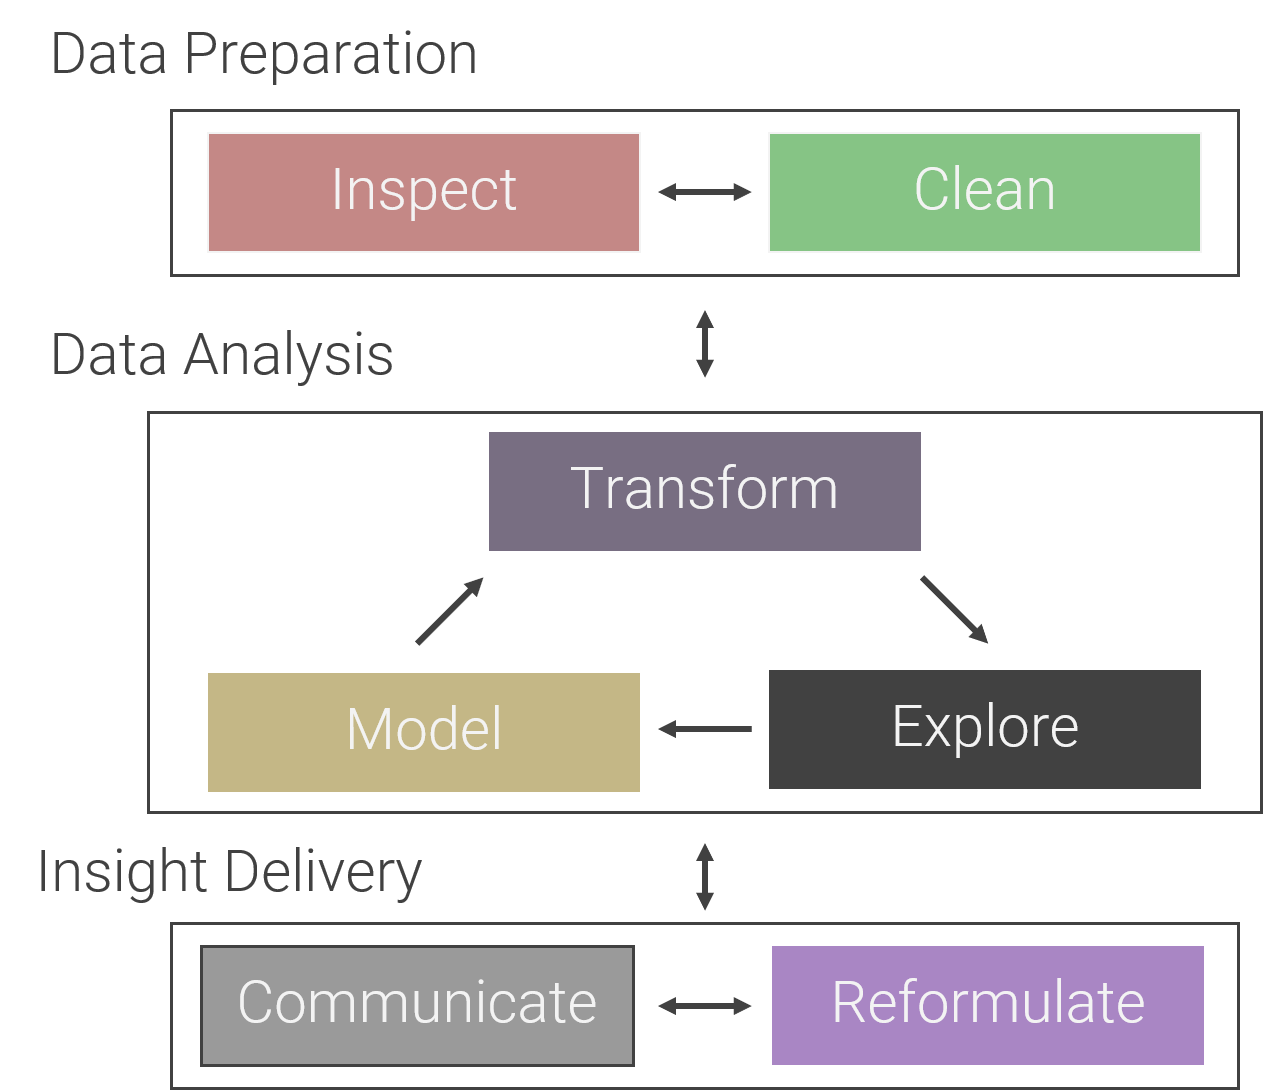
\includegraphics[width=17.54in]{images/data_science_workflow} 

}

\caption{Data scientific workflow.}\label{fig:ds-workflow}
\end{figure}

\hypertarget{data-preparation}{%
\subsection{Data Preparation}\label{data-preparation}}

\hypertarget{inspect}{%
\subsubsection{Inspect}\label{inspect}}

Goal:
Gain familiarity with the data
Key Steps:
Learn collection details
Check data imported correctly
Determine data types
Ascertain consistency and validity
Tabulate and compute other basic summary statistics
Create basic plots of key variables of interest

\hypertarget{clean}{%
\subsubsection{Clean}\label{clean}}

Goal:
Prepare data for analysis
Key Steps:
Remove/correct errors
Make data formatting consistent
Organize text data
Create tidy data (one observation per row)
Organize data into related tables
Document all choices

\hypertarget{data-analysis}{%
\subsection{Data Analysis}\label{data-analysis}}

\hypertarget{transform}{%
\subsubsection{Transform}\label{transform}}

Goal:
Adjust data as needed for analysis
Key Steps:
Create secondary variables
Decorrelate data
Identify latent factors
Engineer new features

\hypertarget{explore}{%
\subsubsection{Explore}\label{explore}}

Goal:
Allow data to suggest hypotheses
Key Steps:
Graphical visualizations
Exploratory analyses
Note:
Caution must be taken to avoid high false discovery rate when using automated tools

\hypertarget{model}{%
\subsubsection{Model}\label{model}}

Goal:
Conduct formal statistical modeling
Key Steps:
Conduct traditional statistical modeling
Build predictive models
Note:
This step may feed back into transform and explore

\hypertarget{insight-delivery}{%
\subsection{Insight Delivery}\label{insight-delivery}}

\hypertarget{communicate}{%
\subsubsection{Communicate}\label{communicate}}

Goal:
Exchange research information
Key Steps:
Automate reporting as much as possible
Share insights
Receive feedback
Note:
Design principles essential to make information accessible

\hypertarget{reformulate}{%
\subsubsection{Reformulate}\label{reformulate}}

Goal:
Incorporate feedback into workflow
Key Steps:
Investigate new questions
Revise communications
Note:
Reformulation make take us back to data cleaning

\hypertarget{benefits-of-data-science}{%
\section{Benefits of Data Science}\label{benefits-of-data-science}}

\hypertarget{reproducible-research}{%
\subsection{Reproducible Research}\label{reproducible-research}}

\begin{itemize}
\tightlist
\item
  Time savings
\item
  Collaboration
\item
  Continuous improvement
\end{itemize}

\hypertarget{data-driven-decision-making}{%
\subsection{Data-Driven Decision Making}\label{data-driven-decision-making}}

\hypertarget{standardized-data-collection}{%
\subsection{Standardized Data Collection}\label{standardized-data-collection}}

\hypertarget{standardized-reporting}{%
\subsection{Standardized Reporting}\label{standardized-reporting}}

\begin{itemize}
\tightlist
\item
  Especially valuable when there are multiple sites globally
\end{itemize}

\hypertarget{improved-business-impact}{%
\subsection{Improved Business Impact}\label{improved-business-impact}}

\hypertarget{how-to-learn-data-science}{%
\section{How to Learn Data Science}\label{how-to-learn-data-science}}

Learning data science is much like learning a language or learning to play an instrument - you have to practice. Our advice based on mentoring many students and clients is to get started sooner rather than later, and to accept that the code you'll write in the future will always be better than the code you'll write today. Also, many of the small details that separate an proficient data scientist from a novice can only really be learned through practice as there are too many small details to learn them all in advice. So, starting today, do your best to write at least some code for all your projects. If a time deadline prevents you from completing the analysis in R, that's fine, but at least gain the experience of making an RStudio project and loading the data in R. Then, as time allows, try to duplicate your analyses in R, being quick to search for solutions when you run into errors. Often simply copying and pasting your error into a search engine will be enough to find the solution to your problem. Moreover, searching for solutions is its own skill that also requires practice. Finally, if you are really stuck, reach out to a colleague (or even the authors of this book) for help

\hypertarget{how-to-use-this-book}{%
\section{How to Use This Book}\label{how-to-use-this-book}}

We recommend following the instructions in Chapter \ref{start-R} to get started.

\hypertarget{common-data-science-tools}{%
\section{Common Data Science Tools}\label{common-data-science-tools}}

\hypertarget{why-r}{%
\section{Why R?}\label{why-r}}

For sensory and consumer scientists, we recommend the R ecosystem of tools for three main reasons. The first reason is cultural - R has from its inception been oriented more towards statistics than to computer science, making the feeling of programming in R more natural (in our experience) for sensory and consumer scientists than programming in Python. This opinion of experience is not to say that a sensory and consumer scientist shouldn't learn Python if they are so inclined, or even that Python tools aren't sometimes superior to R tools (in fact, they sometimes are). This latter point leads to our second reason, which is that R tools are typically better suited to sensory and consumer science than are Python tools. Even when Python tools are superior, the R tools are still sufficient for sensory and consumer science purposes, plus there are many custom packages such as SensR, SensoMineR, and FactorMineR that have been specifically developed for sensory and consumer science. Finally, the recent work by the RStudio company, and especially the exceptional work of Hadley Wickham, has lead to a very low barrier to entry for programming within R together with exceptional tools for data manipulation.

We continue our discussion of getting started with R in the next chapter.

\hypertarget{start-R}{%
\chapter{Getting Started with R}\label{start-R}}

\hypertarget{r}{%
\section{R}\label{r}}

R is an open-source programming language and software environment
First released in 1995, R is an open-source implementation of S
R was developed by Ross Ihaka and Robert Gentleman
The name ``R'' is partly a play on Ihaka's and Gentleman's first names
R is a scripting language (not a compiled language)
Lines of R code run (mostly) in order
R is currently the 7th most popular programming language in the world

\hypertarget{why-learn-a-programming-language}{%
\subsection{Why Learn a Programming Language?}\label{why-learn-a-programming-language}}

Control
Speed
Reduced errors
Increased capability
Continuous improvement
Improved collaboration
Reproducible results

\hypertarget{why-r-1}{%
\subsection{Why R?}\label{why-r-1}}

R originated as a statistical computing language
It has a culture germane to sensory science
R is well-supported with an active community
Extensive online help is available
Many books, courses, and other educational material exist
The universe of available packages is vast
R excels at data manipulation and results reporting
R has more specialized tools for sensory analysis than other programming language

\hypertarget{steps-to-install-r}{%
\subsection{Steps to Install R}\label{steps-to-install-r}}

The first step in this journey is to install R. For this, visit \href{https://www.r-project.org/}{The R Project for Statistical Computing}. From there, follow the download instructions to install R for your particular platform.

\url{https://cran.r-project.org/bin/windows/base/}
Download the latest version of R
Install R with default options
You will almost certainly be running 64-bit R
Note: If you are running R 4.0 or higher, you might need to install Rtools:
\url{https://cran.r-project.org/bin/windows/Rtools/}

\hypertarget{rstudio}{%
\section{RStudio}\label{rstudio}}

\hypertarget{steps-to-install-rstudio}{%
\subsection{Steps to Install RStudio}\label{steps-to-install-rstudio}}

Next you need to install RStudio, which is our recommended integrated development environment (IDE) for developing R code. To do so, visit the \href{https://rstudio.com/products/rstudio/download/}{RStudio desktop download page} and follow the installation instructions.

Once you have installed R and RStudio, you should be able to open RStudio and enter the following into the Console to receive the number ``3'' as your output:

\begin{Shaded}
\begin{Highlighting}[]
\NormalTok{x }\OtherTok{\textless{}{-}} \DecValTok{1}
\NormalTok{y }\OtherTok{\textless{}{-}} \DecValTok{2}

\NormalTok{x }\SpecialCharTok{+}\NormalTok{ y}
\end{Highlighting}
\end{Shaded}

\begin{verbatim}
## [1] 3
\end{verbatim}

Some recommendations upon installing RStudio:

\begin{itemize}
\tightlist
\item
  Change the color scheme to dark.
\item
  Put the console on the right.
\end{itemize}

\url{https://www.rstudio.com/products/rstudio/download/\#download}
Download and install the latest (almost certainly 64-bit) version of RStudio with default options
Adjustments:
Uncheck ``Restore .RData into workspace at startup
Select ``Never'' for ``Save workspace to .RData on exit''
Change color scheme to dark (e.g.~``Idle Fingers'')
Put console on right

\hypertarget{create-a-local-project}{%
\subsection{Create a Local Project}\label{create-a-local-project}}

Always work in an RStudio project
Projects keep your files (and activity) organized
Projects help manage your file path (so your computer can find things)
Projects allow for more advanced capabilities later (like GitHub or renv)
We cover the use of GitHub in a future webinar
For now we create projects locally

\hypertarget{install-and-load-packages}{%
\subsection{Install and Load Packages}\label{install-and-load-packages}}

As you use R, you will want to make use of the many packages others (and perhaps you) have written
Essential packages (or collections):
tidyverse, readxl
Custom Microsoft office document creation
officer, flextable, rvg, openxlsx, extrafont, extrafontdb
Sensory specific packages
sensR , SensoMineR, FactoMineR, factoextra
There are many more, for statistical tests of all varieties, to multivariate analysis, to machine learning, to text analysis, etc.

You only need to install each package once per R version
To install a package, you can:
Type install.packages(``{[}package name{]}'')
Use the RStudio dropdown
In addition, if a script loads package that are not installed, RStudio will prompt you to install the package
Notes:
If you do not have write access on your computer, you might need IT help to install packages
You might need to safelist various R related tools and sites

\hypertarget{run-sample-code}{%
\subsection{Run Sample Code}\label{run-sample-code}}

Like any language, R is best learned first through example then through study
We start with a series of examples to illustrate basic principles
For this example, we analyze a series of Tetrad tests

Suppose you have 15 out of 44 correct in a Tetrad test
Using sensR, it's easy to analyze these data:

\begin{Shaded}
\begin{Highlighting}[]
\FunctionTok{library}\NormalTok{(sensR)}

\NormalTok{num\_correct }\OtherTok{\textless{}{-}} \DecValTok{15}  
\NormalTok{num\_total }\OtherTok{\textless{}{-}} \DecValTok{44}  
  
\NormalTok{discrim\_res }\OtherTok{\textless{}{-}} \FunctionTok{discrim}\NormalTok{(num\_correct, num\_total, }\AttributeTok{method =} \StringTok{"tetrad"}\NormalTok{)  }
  
\FunctionTok{print}\NormalTok{(discrim\_res)  }
\end{Highlighting}
\end{Shaded}

\begin{verbatim}
## 
## Estimates for the tetrad discrimination protocol with 15 correct
## answers in 44 trials. One-sided p-value and 95 % two-sided confidence
## intervals are based on the 'exact' binomial test. 
## 
##         Estimate Std. Error  Lower  Upper
## pc       0.34091    0.07146 0.3333 0.4992
## pd       0.01136    0.10719 0.0000 0.2488
## d-prime  0.20363    0.96585 0.0000 1.0193
## 
## Result of difference test:
## 'exact' binomial test:  p-value = 0.5141 
## Alternative hypothesis: d-prime is greater than 0
\end{verbatim}

\hypertarget{git-and-github}{%
\section{Git and GitHub}\label{git-and-github}}

Git is a version control system that allows you to revert to earlier versions of your code, if necessary. GitHub is service that allows for online backups of your code and which facilitates collaboration between team members. We highly recommend that you integrate both Git and GitHub into your data scientific workflow. For a full review of Git and GitHub from an R programming perspective, we recommend \href{https://happygitwithr.com/}{Happy Git with R} by Jenny Bryant. In what follows, we simply provide the minimum information needed to get you up and running with Git and GitHub. Also, for an insightful discussion of the need for version control, please see (\citet{bryan2018excuse}).

\hypertarget{git}{%
\subsection{Git}\label{git}}

\begin{itemize}
\tightlist
\item
  Install Git

  \begin{itemize}
  \tightlist
  \item
    Windows
  \item
    macOS
  \end{itemize}
\item
  Register with RStudio
\end{itemize}

\hypertarget{github}{%
\subsection{GitHub}\label{github}}

\begin{itemize}
\tightlist
\item
  Create a GitHub account
\item
  Register with RStudio
\end{itemize}

\hypertarget{part-data-scientific-workflow}{%
\part*{Data Scientific Workflow}\label{part-data-scientific-workflow}}
\addcontentsline{toc}{part}{Data Scientific Workflow}

\hypertarget{ex_proj}{%
\chapter{Example Project}\label{ex_proj}}

\hypertarget{background}{%
\section{Background}\label{background}}

\hypertarget{other-details}{%
\section{Other details}\label{other-details}}

\hypertarget{conclusions}{%
\section{Conclusions?}\label{conclusions}}

\hypertarget{data_prep}{%
\chapter{Data Preparation}\label{data_prep}}

To analyze data, one need \emph{data}. If this data is already available in R, then the analysis can be performed directly. However, in much cases, the data is stored outside the R environment, and needs to be imported.

\hypertarget{data-importation}{%
\section{Data Importation}\label{data-importation}}

In practice, the data might be stored in as many format as one can imagine, whether it ends up being a fairly common solution (.txt file, .csv file, or .xls/.xlsx file), or software specific (e.g.~Stata, SPSS, etc.).
Since it is very common to store the data in Excel spreadsheets (.xlsx) due to its simplicity, the emphasis is on this solution. Fortunately, most generalities presented for Excel files also apply to other formats through \texttt{base::read.table()} for .txt files, \texttt{base::read.csv()} and \texttt{base::read.csv2()} for .csv files, or through the \texttt{\{read\}} package (which is part of the \texttt{\{tidyverse\}}).

For other (less common) formats, the reader can find packages that would allow importing their files into R. Particular interest can be given to the package \texttt{\{rio\}} (\emph{rio} stands for \emph{R} \emph{I}nput and \emph{O}utput) which provides an easy solution that 1. can handle a large variety of files, 2. can actually guess the type of file it is, and 3. provides tools to import, export, and convert almost any type of data format, including .csv, .xls and .xlsx, or data from other statistical software such as SAS (.sas7bdat and .xpt), SPSS (.sav and .por), or Stata (.dta). As an alternative, the package \texttt{\{foreign\}} provides functions that allow importing data stored from other statistical software (incl.~Minitab, S, SAS, Stata, SPSS, etc.)

Although Excel is most likely one of the most popular way of storing data, there are no \texttt{\{base\}} functions that allow importing such files easily. Fortunately, many packages have been developed in that purpose, including \texttt{\{XLConnect\}}, \texttt{\{xlsx\}}, \texttt{\{gdata\}}, and \texttt{\{readxl\}}. Due to its convenience and speed of execution, we will be using \texttt{\{readxl\}} here.

\hypertarget{importing-structured-excel-file}{%
\subsection{Importing Structured Excel File}\label{importing-structured-excel-file}}

First, let's import the \emph{Sensory Profile.xlsx} workbook using the \texttt{readxl::read\_xlsx()} file, by informing as parameter the location of the file (informed in \texttt{file\_path} using the package \texttt{\{here\}}) and the \texttt{sheet} we want to read from.

This file is called \emph{structured} as all the relevant information is already stored in the same sheet in a structured way. In other words, no decoding is required here, and there are no `unexpected' rows or columns (e.g.~empty lines, or lines with additional information regarding the data but that is not data):

\begin{itemize}
\tightlist
\item
  The first row within the \emph{Data} sheet of \emph{Sensory Profile.xlsx} contains the headers,\\
\item
  From the second row onwards, only data is being stored.
\end{itemize}

Since this data will be used for some analyses, it is assigned data to an R object called \texttt{sensory}.

\begin{Shaded}
\begin{Highlighting}[]
\FunctionTok{library}\NormalTok{(here)}
\end{Highlighting}
\end{Shaded}

\begin{verbatim}
## here() starts at C:/Aigora/books/intro to data science/i2ds4scc_bookdown
\end{verbatim}

\begin{Shaded}
\begin{Highlighting}[]
\NormalTok{file\_path }\OtherTok{\textless{}{-}} \FunctionTok{here}\NormalTok{(}\StringTok{"data"}\NormalTok{,}\StringTok{"Sensory Profile.xlsx"}\NormalTok{) }

\FunctionTok{library}\NormalTok{(readxl)}
\NormalTok{sensory }\OtherTok{\textless{}{-}} \FunctionTok{read\_xlsx}\NormalTok{(file\_path, }\AttributeTok{sheet=}\StringTok{"Data"}\NormalTok{)}
\end{Highlighting}
\end{Shaded}

To ensure that the importation went well, we print \texttt{sensory} to see how it looks like. Since \texttt{\{readxl\}} has been developed by Hadley Wickham and colleagues, its functions follow the \texttt{\{tidyverse\}} principles and the dataset thus imported is a \texttt{tibble}. Let's take advantage of the printing properties of a \texttt{tibble} to evaluate \texttt{sensory}:

\begin{Shaded}
\begin{Highlighting}[]
\NormalTok{sensory}
\end{Highlighting}
\end{Shaded}

\begin{verbatim}
## # A tibble: 99 x 35
##    Judge Code  Product Shiny `External color~ `Color evenness` `Qtt of inclusi~
##    <chr> <chr> <chr>   <dbl>            <dbl>            <dbl>            <dbl>
##  1 J01   B     12GP_f   48.6             30               13.2             10.8
##  2 J01   D     12GP16~  46.2             45.6             37.8              0  
##  3 J01   C     12GP23~  48               45.6             17.4              7.8
##  4 J01   G     12SA_f    5.4              6.6             17.4              0  
##  5 J01   I     12SA23~   0               42.6             18               21  
##  6 J01   E     16PPK_p   0               23.4             49.2              0  
##  7 J01   New   23pK_p    4.8             33.6             15.6             32.4
##  8 J01   H     23PLK_p   0               51.6             48.6             23.4
##  9 J01   F     29PPK_p   0               50.4             24               27.6
## 10 J01   A     ck1      52.8             30               22.8              9.6
## # ... with 89 more rows, and 28 more variables: `Surface defects` <dbl>, `Print
## #   quality` <dbl>, Thickness <dbl>, `Color constrast` <dbl>, `Overall odor
## #   intensity` <dbl>, `Fatty odor` <dbl>, `Roasted odor` <dbl>, `Cereal
## #   flavor` <dbl>, `Raw dough flavor` <dbl>, `Fatty flavor` <dbl>, `Dairy
## #   flavor` <dbl>, `Roasted flavor` <dbl>, `Overall flavor persistence` <dbl>,
## #   Salty <dbl>, Sweet <dbl>, Sour <dbl>, Bitter <dbl>, Astringent <dbl>,
## #   Warming <dbl>, `Initial hardness` <dbl>, Brittle <dbl>, Crunchy <dbl>,
## #   `Fatty in mouth` <dbl>, Light <dbl>, `Dry in mouth` <dbl>, `Qtt of
## #   inclusions in mouth` <dbl>, Sticky <dbl>, Melting <dbl>
\end{verbatim}

\texttt{sensory} is a tibble with 99 rows and 35 columns that includes the \texttt{Judge} information (first column, defined as character), the \texttt{Product} information (second and third columns, defined as character), and the sensory attributes (fourth column onward, defined as numerical or \texttt{dbl}).

Additionally, we can also print a \texttt{summary()} of \texttt{sensory} to get some extra information regarding the data (such as the minimum, maximum, mean and median for each numerical variable)"

\begin{Shaded}
\begin{Highlighting}[]
\FunctionTok{summary}\NormalTok{(sensory)}
\end{Highlighting}
\end{Shaded}

\begin{verbatim}
##     Judge               Code             Product              Shiny     
##  Length:99          Length:99          Length:99          Min.   : 0.0  
##  Class :character   Class :character   Class :character   1st Qu.: 9.3  
##  Mode  :character   Mode  :character   Mode  :character   Median :21.0  
##                                                           Mean   :23.9  
##                                                           3rd Qu.:38.4  
##                                                           Max.   :54.0  
##  External color intensity Color evenness  Qtt of inclusions Surface defects
##  Min.   : 6.60            Min.   : 6.60   Min.   : 0.00     Min.   : 4.80  
##  1st Qu.:27.00            1st Qu.:19.50   1st Qu.:13.80     1st Qu.:15.30  
##  Median :34.80            Median :26.40   Median :19.80     Median :21.00  
##  Mean   :33.68            Mean   :28.19   Mean   :20.63     Mean   :23.35  
##  3rd Qu.:42.60            3rd Qu.:37.20   3rd Qu.:29.10     3rd Qu.:30.60  
##  Max.   :55.20            Max.   :53.40   Max.   :40.80     Max.   :51.60  
##  Print quality     Thickness     Color constrast Overall odor intensity
##  Min.   :12.00   Min.   : 7.80   Min.   : 5.40   Min.   : 0.00         
##  1st Qu.:36.30   1st Qu.:18.30   1st Qu.:21.00   1st Qu.:10.20         
##  Median :40.80   Median :25.80   Median :32.40   Median :18.00         
##  Mean   :40.72   Mean   :25.48   Mean   :30.02   Mean   :18.67         
##  3rd Qu.:47.10   3rd Qu.:32.10   3rd Qu.:40.20   3rd Qu.:26.10         
##  Max.   :60.00   Max.   :52.80   Max.   :51.60   Max.   :40.20         
##    Fatty odor     Roasted odor   Cereal flavor   Raw dough flavor
##  Min.   : 0.00   Min.   : 0.00   Min.   : 0.00   Min.   : 0.00   
##  1st Qu.: 0.00   1st Qu.: 8.10   1st Qu.:18.00   1st Qu.: 3.00   
##  Median : 5.40   Median :15.00   Median :25.20   Median :13.20   
##  Mean   : 6.81   Mean   :15.07   Mean   :24.99   Mean   :14.23   
##  3rd Qu.:10.50   3rd Qu.:20.70   3rd Qu.:31.20   3rd Qu.:24.60   
##  Max.   :27.00   Max.   :42.00   Max.   :48.00   Max.   :43.20   
##   Fatty flavor     Dairy flavor    Roasted flavor  Overall flavor persistence
##  Min.   : 0.000   Min.   : 0.000   Min.   : 0.00   Min.   : 0.00             
##  1st Qu.: 0.000   1st Qu.: 0.000   1st Qu.: 9.00   1st Qu.:16.20             
##  Median : 6.600   Median : 7.200   Median :17.40   Median :22.80             
##  Mean   : 7.419   Mean   : 9.106   Mean   :17.68   Mean   :22.73             
##  3rd Qu.:13.200   3rd Qu.:13.500   3rd Qu.:24.60   3rd Qu.:28.80             
##  Max.   :24.000   Max.   :46.800   Max.   :51.60   Max.   :43.80             
##      Salty            Sweet            Sour            Bitter      
##  Min.   : 0.000   Min.   : 0.00   Min.   : 0.000   Min.   : 0.000  
##  1st Qu.: 0.000   1st Qu.: 9.90   1st Qu.: 0.000   1st Qu.: 0.000  
##  Median : 1.200   Median :18.00   Median : 0.000   Median : 7.800  
##  Mean   : 5.027   Mean   :17.82   Mean   : 1.461   Mean   : 8.103  
##  3rd Qu.:10.050   3rd Qu.:24.30   3rd Qu.: 0.000   3rd Qu.:14.100  
##  Max.   :19.200   Max.   :43.20   Max.   :13.800   Max.   :27.600  
##    Astringent       Warming      Initial hardness    Brittle     
##  Min.   : 0.00   Min.   : 0.00   Min.   : 0.00    Min.   : 0.00  
##  1st Qu.: 0.00   1st Qu.: 9.30   1st Qu.:19.50    1st Qu.:27.60  
##  Median : 8.40   Median :16.80   Median :30.60    Median :34.80  
##  Mean   :11.45   Mean   :16.76   Mean   :30.12    Mean   :31.77  
##  3rd Qu.:19.50   3rd Qu.:25.20   3rd Qu.:39.30    3rd Qu.:39.14  
##  Max.   :34.20   Max.   :47.40   Max.   :60.00    Max.   :57.00  
##     Crunchy      Fatty in mouth      Light        Dry in mouth  
##  Min.   : 8.40   Min.   : 0.00   Min.   : 5.40   Min.   :11.40  
##  1st Qu.:23.25   1st Qu.: 0.00   1st Qu.:22.80   1st Qu.:39.00  
##  Median :30.60   Median : 5.40   Median :31.80   Median :45.00  
##  Mean   :29.62   Mean   : 7.32   Mean   :30.21   Mean   :42.99  
##  3rd Qu.:36.30   3rd Qu.:12.90   3rd Qu.:37.20   3rd Qu.:49.80  
##  Max.   :48.60   Max.   :27.00   Max.   :53.40   Max.   :58.80  
##  Qtt of inclusions in mouth     Sticky         Melting    
##  Min.   : 0.00              Min.   : 6.00   Min.   : 0.0  
##  1st Qu.:15.90              1st Qu.:27.00   1st Qu.:13.2  
##  Median :26.40              Median :33.60   Median :19.2  
##  Mean   :24.92              Mean   :32.73   Mean   :20.5  
##  3rd Qu.:35.40              3rd Qu.:39.60   3rd Qu.:27.3  
##  Max.   :45.60              Max.   :52.80   Max.   :38.4
\end{verbatim}

At last, we can list the structure of the dataset through the \texttt{str()} function.

\begin{Shaded}
\begin{Highlighting}[]
\FunctionTok{str}\NormalTok{(sensory)}
\end{Highlighting}
\end{Shaded}

\begin{verbatim}
## tibble [99 x 35] (S3: tbl_df/tbl/data.frame)
##  $ Judge                     : chr [1:99] "J01" "J01" "J01" "J01" ...
##  $ Code                      : chr [1:99] "B" "D" "C" "G" ...
##  $ Product                   : chr [1:99] "12GP_f" "12GP16PSL_m" "12GP23P_m" "12SA_f" ...
##  $ Shiny                     : num [1:99] 48.6 46.2 48 5.4 0 0 4.8 0 0 52.8 ...
##  $ External color intensity  : num [1:99] 30 45.6 45.6 6.6 42.6 23.4 33.6 51.6 50.4 30 ...
##  $ Color evenness            : num [1:99] 13.2 37.8 17.4 17.4 18 49.2 15.6 48.6 24 22.8 ...
##  $ Qtt of inclusions         : num [1:99] 10.8 0 7.8 0 21 0 32.4 23.4 27.6 9.6 ...
##  $ Surface defects           : num [1:99] 13.2 48.6 14.4 36 36 12.6 13.8 18 39.6 22.8 ...
##  $ Print quality             : num [1:99] 54 45.6 49.2 42.6 51 47.4 43.8 45.6 53.4 48.6 ...
##  $ Thickness                 : num [1:99] 35.4 43.2 25.8 32.4 31.8 29.4 36 31.2 36 38.4 ...
##  $ Color constrast           : num [1:99] 40.2 45.6 17.4 41.4 41.4 12.6 36 5.4 21 37.8 ...
##  $ Overall odor intensity    : num [1:99] 24.6 7.2 21.6 13.8 26.4 18 16.2 13.8 0 16.8 ...
##  $ Fatty odor                : num [1:99] 5.4 0 0 0 6.6 8.4 7.8 7.8 0 6.6 ...
##  $ Roasted odor              : num [1:99] 20.4 6 18.6 16.2 16.8 16.2 16.2 12.6 7.2 15.6 ...
##  $ Cereal flavor             : num [1:99] 25.8 16.2 30 18 28.8 21.6 23.4 23.4 28.8 24.6 ...
##  $ Raw dough flavor          : num [1:99] 28.8 28.2 26.4 21 26.4 27.6 31.2 27 27.6 28.2 ...
##  $ Fatty flavor              : num [1:99] 7.2 0 0 6 7.2 6.6 10.8 7.2 0 13.8 ...
##  $ Dairy flavor              : num [1:99] 0 0 0 0 0 0 4.8 0 0 0 ...
##  $ Roasted flavor            : num [1:99] 19.2 28.2 27 21.6 25.8 20.4 26.4 24.6 22.2 24.6 ...
##  $ Overall flavor persistence: num [1:99] 24.6 14.4 25.2 18 22.8 21 24 21.6 25.2 23.4 ...
##  $ Salty                     : num [1:99] 0 0 0 0 0 0 3.6 0 0 0 ...
##  $ Sweet                     : num [1:99] 19.2 11.4 9.6 10.8 21 20.4 21 10.2 21 13.8 ...
##  $ Sour                      : num [1:99] 0 0 0 0 0 0 0.6 0 0 0 ...
##  $ Bitter                    : num [1:99] 21.6 9 21 0 22.8 8.4 27.6 9.6 18.6 19.2 ...
##  $ Astringent                : num [1:99] 0 18.6 25.8 21 26.4 16.2 31.8 23.4 25.2 0 ...
##  $ Warming                   : num [1:99] 0 0 13.8 10.8 15 0 27.6 19.8 14.4 0 ...
##  $ Initial hardness          : num [1:99] 17.4 19.8 33 10.2 29.4 16.2 18 34.2 28.2 11.4 ...
##  $ Brittle                   : num [1:99] 35.4 33.6 27.6 29.4 34.8 38.4 35.4 35.4 33 39.6 ...
##  $ Crunchy                   : num [1:99] 32.4 28.8 25.2 27 32.4 35.4 34.8 30.6 27.6 25.8 ...
##  $ Fatty in mouth            : num [1:99] 9.6 9.6 6 5.4 12 7.2 14.4 5.4 0 0 ...
##  $ Light                     : num [1:99] 21 40.5 20.4 25.8 21 ...
##  $ Dry in mouth              : num [1:99] 25.8 28.2 31.2 22.2 27.6 34.2 31.8 37.8 33.6 27 ...
##  $ Qtt of inclusions in mouth: num [1:99] 22.2 13.2 10.2 9 29.4 18 31.2 25.8 26.4 27.6 ...
##  $ Sticky                    : num [1:99] 35.4 21.6 37.2 22.8 37.2 39 34.2 36.6 36 37.2 ...
##  $ Melting                   : num [1:99] 36 34.2 8.4 34.8 19.8 34.8 36.6 19.2 21.6 33.6 ...
\end{verbatim}

This function provides an overview of the first element of each variables (and the format they are in) as a list, and allows the user to have a first scan to eventually detect \emph{errors} or \emph{mishaps} during the importation.

Here, the data has been imported as expected.

\hypertarget{importing-unstructured-excel-file}{%
\subsection{Importing Unstructured Excel File}\label{importing-unstructured-excel-file}}

In some cases, the dataset is not so well organized/structured, and may need to be \emph{decoded}. This is the case for the workbook entitled \emph{TFEQ.xlsx}. For this file:

\begin{itemize}
\tightlist
\item
  The variables' name have been coded and their corresponding names (together with some other valuable information we will be using in the next chapter) are stored in a different sheet entitled \emph{Variables};
\item
  The different levels of each variable (including their code and corresponding names) are stored in another sheet entitled \emph{Levels}.
\end{itemize}

To import and decode this dataset, multiple steps are required:

\begin{itemize}
\tightlist
\item
  Import the variables' name only;
\item
  Import the information regarding the levels;
\item
  Import the dataset without the first line of header, but by providing the correct names obtained in the first step;
\item
  Decode each question (when needed) by replacing the numerical code by their corresponding labels.
\end{itemize}

Let's start with importing the variables' names from \emph{TFEQ.xlsx} (sheet \emph{Variables})

\begin{Shaded}
\begin{Highlighting}[]
\NormalTok{file\_path }\OtherTok{\textless{}{-}} \FunctionTok{here}\NormalTok{(}\StringTok{"data"}\NormalTok{,}\StringTok{"TFEQ.xlsx"}\NormalTok{) }

\NormalTok{var\_names }\OtherTok{\textless{}{-}} \FunctionTok{read\_xlsx}\NormalTok{(file\_path, }\AttributeTok{sheet=}\StringTok{"Variables"}\NormalTok{)}
\NormalTok{var\_names}
\end{Highlighting}
\end{Shaded}

\begin{verbatim}
## # A tibble: 62 x 6
##    Code  `Original Questions (French)`  Name     Direction Value `Full Question`
##    <chr> <chr>                          <chr>    <chr>     <dbl> <chr>          
##  1 Q1    Où habitez-vous?               Living ~ <NA>         NA <NA>           
##  2 Q2    Comment habitez-vous?          Housing  <NA>         NA <NA>           
##  3 Q3    N° Juge                        Judge    <NA>         NA <NA>           
##  4 Q4    Quelle est votre taille (en m~ Height   <NA>         NA <NA>           
##  5 Q5    Quel est votre poids?          Weight   <NA>         NA <NA>           
##  6 Q6    IMC                            BMI      <NA>         NA <NA>           
##  7 Q7    Quelle est votre situation ma~ Marital~ <NA>         NA <NA>           
##  8 Q8    Nombre de personnes vivant au~ Househo~ <NA>         NA <NA>           
##  9 Q9    Dans quelle tranche de revenu~ Income ~ <NA>         NA <NA>           
## 10 Q10   Dans quelle catégorie sociopr~ Occupat~ <NA>         NA <NA>           
## # ... with 52 more rows
\end{verbatim}

In a similar way, let's import the information related to the levels of each variable, stored in the \emph{Levels} sheet.
A deeper look at the \emph{Levels} sheet shows that only the coded names of the variables are available. In order to include the final names, \texttt{var\_names} is joined (using \texttt{inner\_join}).

\begin{Shaded}
\begin{Highlighting}[]
\FunctionTok{library}\NormalTok{(tidyverse)}
\end{Highlighting}
\end{Shaded}

\begin{verbatim}
## -- Attaching packages --------------------------------------- tidyverse 1.3.0 --
\end{verbatim}

\begin{verbatim}
## v ggplot2 3.3.2     v purrr   0.3.4
## v tibble  3.0.4     v dplyr   1.0.2
## v tidyr   1.1.2     v stringr 1.4.0
## v readr   1.4.0     v forcats 0.5.0
\end{verbatim}

\begin{verbatim}
## -- Conflicts ------------------------------------------ tidyverse_conflicts() --
## x dplyr::filter() masks stats::filter()
## x dplyr::lag()    masks stats::lag()
\end{verbatim}

\begin{Shaded}
\begin{Highlighting}[]
\NormalTok{var\_labels }\OtherTok{\textless{}{-}} \FunctionTok{read\_xlsx}\NormalTok{(file\_path, }\AttributeTok{sheet=}\StringTok{"Levels"}\NormalTok{) }\SpecialCharTok{\%\textgreater{}\%} 
  \FunctionTok{inner\_join}\NormalTok{(dplyr}\SpecialCharTok{::}\FunctionTok{select}\NormalTok{(var\_names, Code, Name), }\AttributeTok{by=}\FunctionTok{c}\NormalTok{(}\AttributeTok{Question=}\StringTok{"Code"}\NormalTok{))}

\NormalTok{var\_labels}
\end{Highlighting}
\end{Shaded}

\begin{verbatim}
## # A tibble: 172 x 5
##    Question  Code `Original Levels (French)` Levels            Name          
##    <chr>    <dbl> <chr>                      <chr>             <chr>         
##  1 Q1           1 Zone urbaine               Urban Area        Living area   
##  2 Q1           2 Zone rurbaine              Rurban Area       Living area   
##  3 Q1           3 Zone rurale                Rural Area        Living area   
##  4 Q2           1 Appartement                Apartment         Housing       
##  5 Q2           2 Maison individuelle        House             Housing       
##  6 Q7           1 Divorcé(e)                 Divorced          Marital status
##  7 Q7           2 Marié(e)                   Married           Marital status
##  8 Q7           3 Vivant maritalement        Conjugal          Marital status
##  9 Q7           4 Célibataire                Single            Marital status
## 10 Q7           5 Pacsé(e)                   Civil Partnership Marital status
## # ... with 162 more rows
\end{verbatim}

\textbf{Note}: In some cases, this information is directly available in the dataset as sub-header: A solution is then to import the first rows of the dataset that contain this information using the parameter \texttt{n\_max} from `readxl::read\_xlsx``. For each variable (when information is available), store that information as a list of tables that contains the code and their corresponding label.

\textbf{THIS SECTION BELOW MIGHT NEED TO GET PASSED ON TO THE EXERCISE}

Since most likely this system of coding follow a fixed pattern, we strongly recommend the use of \texttt{\{tidytext\}} and its function \texttt{unnest\_tokens()}.
For example, let's imagine that the our information is structured as \emph{code1=label1,code2=label2,\ldots{}} (e.g.~\emph{0=No,1=Yes}). In such case, first use \texttt{unnest\_tokens()} to split this string by `,'. This creates a tibble with as many rows as there are \emph{code=label} and one column. Next, split this column into two columns using \texttt{separate()} and \texttt{sep="="}.

\textbf{(PREVIOUS PART) TO BE GIVEN AS AN EXAMPLE/EXERCISE}

Finally, we import the dataset (\emph{Data}) by substituting the coded names with their real names.
To do so, we skip reading the first line (\texttt{skip=1}) that contains the coded names, and force the column names to be defined by \texttt{Name} from \texttt{var\_names} (after ensuring that the names' sequence perfectly match across the two tables!).

\begin{Shaded}
\begin{Highlighting}[]
\NormalTok{TFEQ\_data }\OtherTok{\textless{}{-}} \FunctionTok{read\_xlsx}\NormalTok{(file\_path, }\AttributeTok{sheet=}\StringTok{"Data"}\NormalTok{, }\AttributeTok{col\_names=}\NormalTok{var\_names}\SpecialCharTok{$}\NormalTok{Name, }\AttributeTok{skip=}\DecValTok{1}\NormalTok{)}
\FunctionTok{summary}\NormalTok{(TFEQ\_data)}
\end{Highlighting}
\end{Shaded}

\begin{verbatim}
##   Living area       Housing         Judge               Height     
##  Min.   :1.000   Min.   :1.000   Length:107         Min.   :1.450  
##  1st Qu.:1.000   1st Qu.:1.000   Class :character   1st Qu.:1.600  
##  Median :1.000   Median :2.000   Mode  :character   Median :1.630  
##  Mean   :1.542   Mean   :1.682                      Mean   :1.634  
##  3rd Qu.:2.000   3rd Qu.:2.000                      3rd Qu.:1.680  
##  Max.   :3.000   Max.   :2.000                      Max.   :1.800  
##      Weight           BMI        Marital status  Household size 
##  Min.   :43.00   Min.   :17.63   Min.   :1.000   Min.   :0.000  
##  1st Qu.:53.50   1st Qu.:20.30   1st Qu.:2.000   1st Qu.:2.000  
##  Median :58.00   Median :21.63   Median :3.000   Median :3.000  
##  Mean   :58.25   Mean   :21.79   Mean   :2.944   Mean   :2.944  
##  3rd Qu.:62.35   3rd Qu.:23.33   3rd Qu.:4.000   3rd Qu.:4.000  
##  Max.   :82.00   Max.   :26.47   Max.   :7.000   Max.   :6.000  
##   Income range     Occupation     Highest degree       D1       
##  Min.   :1.000   Min.   : 1.000   Min.   :1.00   Min.   :0.000  
##  1st Qu.:2.000   1st Qu.: 2.000   1st Qu.:2.00   1st Qu.:0.000  
##  Median :2.000   Median : 6.000   Median :3.00   Median :0.000  
##  Mean   :2.421   Mean   : 6.486   Mean   :2.71   Mean   :0.215  
##  3rd Qu.:3.000   3rd Qu.: 9.000   3rd Qu.:4.00   3rd Qu.:0.000  
##  Max.   :4.000   Max.   :17.000   Max.   :6.00   Max.   :1.000  
##        D2               H1              R1               H2        
##  Min.   :0.0000   Min.   :0.000   Min.   :0.0000   Min.   :0.0000  
##  1st Qu.:0.0000   1st Qu.:0.000   1st Qu.:0.0000   1st Qu.:0.0000  
##  Median :1.0000   Median :0.000   Median :0.0000   Median :1.0000  
##  Mean   :0.5794   Mean   :0.243   Mean   :0.4579   Mean   :0.5514  
##  3rd Qu.:1.0000   3rd Qu.:0.000   3rd Qu.:1.0000   3rd Qu.:1.0000  
##  Max.   :1.0000   Max.   :1.000   Max.   :1.0000   Max.   :1.0000  
##        R2               D3               H3               D4        
##  Min.   :0.0000   Min.   :0.0000   Min.   :0.0000   Min.   :0.0000  
##  1st Qu.:0.0000   1st Qu.:0.5000   1st Qu.:0.0000   1st Qu.:0.0000  
##  Median :0.0000   Median :1.0000   Median :0.0000   Median :1.0000  
##  Mean   :0.2991   Mean   :0.7477   Mean   :0.3738   Mean   :0.5607  
##  3rd Qu.:1.0000   3rd Qu.:1.0000   3rd Qu.:1.0000   3rd Qu.:1.0000  
##  Max.   :1.0000   Max.   :1.0000   Max.   :1.0000   Max.   :1.0000  
##        R3               D5               H4              D6        
##  Min.   :0.0000   Min.   :0.0000   Min.   :0.000   Min.   :0.0000  
##  1st Qu.:0.0000   1st Qu.:0.0000   1st Qu.:0.000   1st Qu.:0.0000  
##  Median :1.0000   Median :0.0000   Median :0.000   Median :0.0000  
##  Mean   :0.5327   Mean   :0.3551   Mean   :0.486   Mean   :0.3458  
##  3rd Qu.:1.0000   3rd Qu.:1.0000   3rd Qu.:1.000   3rd Qu.:1.0000  
##  Max.   :1.0000   Max.   :1.0000   Max.   :1.000   Max.   :1.0000  
##        R4               D7               D8               H5        
##  Min.   :0.0000   Min.   :0.0000   Min.   :0.0000   Min.   :0.0000  
##  1st Qu.:0.0000   1st Qu.:0.0000   1st Qu.:0.0000   1st Qu.:0.0000  
##  Median :0.0000   Median :0.0000   Median :1.0000   Median :1.0000  
##  Mean   :0.4486   Mean   :0.3178   Mean   :0.5047   Mean   :0.6168  
##  3rd Qu.:1.0000   3rd Qu.:1.0000   3rd Qu.:1.0000   3rd Qu.:1.0000  
##  Max.   :1.0000   Max.   :1.0000   Max.   :1.0000   Max.   :1.0000  
##        R5               H6               D9               R6        
##  Min.   :0.0000   Min.   :0.0000   Min.   :0.0000   Min.   :0.0000  
##  1st Qu.:0.0000   1st Qu.:0.0000   1st Qu.:0.0000   1st Qu.:0.0000  
##  Median :0.0000   Median :1.0000   Median :1.0000   Median :1.0000  
##  Mean   :0.4486   Mean   :0.5888   Mean   :0.5701   Mean   :0.5421  
##  3rd Qu.:1.0000   3rd Qu.:1.0000   3rd Qu.:1.0000   3rd Qu.:1.0000  
##  Max.   :1.0000   Max.   :1.0000   Max.   :1.0000   Max.   :1.0000  
##        H7               R7               H8              D10        
##  Min.   :0.0000   Min.   :0.0000   Min.   :0.0000   Min.   :0.0000  
##  1st Qu.:0.0000   1st Qu.:0.0000   1st Qu.:0.0000   1st Qu.:0.0000  
##  Median :0.0000   Median :0.0000   Median :0.0000   Median :0.0000  
##  Mean   :0.3271   Mean   :0.2523   Mean   :0.2243   Mean   :0.4206  
##  3rd Qu.:1.0000   3rd Qu.:0.5000   3rd Qu.:0.0000   3rd Qu.:1.0000  
##  Max.   :1.0000   Max.   :1.0000   Max.   :1.0000   Max.   :1.0000  
##        H9              D11              R8              H10       
##  Min.   :0.0000   Min.   :0.000   Min.   :0.0000   Min.   :0.000  
##  1st Qu.:0.0000   1st Qu.:0.000   1st Qu.:0.0000   1st Qu.:0.000  
##  Median :0.0000   Median :0.000   Median :0.0000   Median :0.000  
##  Mean   :0.1963   Mean   :0.486   Mean   :0.1963   Mean   :0.243  
##  3rd Qu.:0.0000   3rd Qu.:1.000   3rd Qu.:0.0000   3rd Qu.:0.000  
##  Max.   :1.0000   Max.   :1.000   Max.   :1.0000   Max.   :1.000  
##        R9             D12              R10              R11        
##  Min.   :0.000   Min.   :0.0000   Min.   :0.0000   Min.   :0.0000  
##  1st Qu.:0.000   1st Qu.:0.0000   1st Qu.:0.0000   1st Qu.:0.0000  
##  Median :1.000   Median :0.0000   Median :0.0000   Median :0.0000  
##  Mean   :0.514   Mean   :0.2617   Mean   :0.1028   Mean   :0.4206  
##  3rd Qu.:1.000   3rd Qu.:1.0000   3rd Qu.:0.0000   3rd Qu.:1.0000  
##  Max.   :1.000   Max.   :1.0000   Max.   :1.0000   Max.   :1.0000  
##       H11              R12              D13              R13       
##  Min.   :0.0000   Min.   :0.0000   Min.   :0.0000   Min.   :1.000  
##  1st Qu.:0.0000   1st Qu.:0.0000   1st Qu.:0.0000   1st Qu.:1.000  
##  Median :0.0000   Median :1.0000   Median :0.0000   Median :1.000  
##  Mean   :0.1589   Mean   :0.7103   Mean   :0.1028   Mean   :1.533  
##  3rd Qu.:0.0000   3rd Qu.:1.0000   3rd Qu.:0.0000   3rd Qu.:2.000  
##  Max.   :1.0000   Max.   :1.0000   Max.   :1.0000   Max.   :4.000  
##       R14             H12             R15             H13       
##  Min.   :1.000   Min.   :1.000   Min.   :1.000   Min.   :1.000  
##  1st Qu.:2.000   1st Qu.:1.500   1st Qu.:2.000   1st Qu.:1.000  
##  Median :3.000   Median :2.000   Median :2.000   Median :2.000  
##  Mean   :2.589   Mean   :1.935   Mean   :2.121   Mean   :2.084  
##  3rd Qu.:3.000   3rd Qu.:2.000   3rd Qu.:3.000   3rd Qu.:3.000  
##  Max.   :4.000   Max.   :4.000   Max.   :4.000   Max.   :4.000  
##       R16             R17             R18             D14       
##  Min.   :2.000   Min.   :1.000   Min.   :1.000   Min.   :1.000  
##  1st Qu.:3.000   1st Qu.:2.000   1st Qu.:1.000   1st Qu.:1.000  
##  Median :3.000   Median :2.000   Median :2.000   Median :2.000  
##  Mean   :3.252   Mean   :2.439   Mean   :1.869   Mean   :1.692  
##  3rd Qu.:4.000   3rd Qu.:3.000   3rd Qu.:2.000   3rd Qu.:2.000  
##  Max.   :4.000   Max.   :4.000   Max.   :4.000   Max.   :3.000  
##       R19             H14             R20             D15       
##  Min.   :1.000   Min.   :1.000   Min.   :1.000   Min.   :1.000  
##  1st Qu.:1.000   1st Qu.:2.000   1st Qu.:1.000   1st Qu.:1.000  
##  Median :1.000   Median :3.000   Median :2.000   Median :2.000  
##  Mean   :1.542   Mean   :2.579   Mean   :1.841   Mean   :1.991  
##  3rd Qu.:2.000   3rd Qu.:4.000   3rd Qu.:2.000   3rd Qu.:3.000  
##  Max.   :4.000   Max.   :4.000   Max.   :4.000   Max.   :4.000  
##       R21             D16       
##  Min.   :0.000   Min.   :1.000  
##  1st Qu.:1.000   1st Qu.:1.000  
##  Median :2.000   Median :2.000  
##  Mean   :2.215   Mean   :1.785  
##  3rd Qu.:3.000   3rd Qu.:2.000  
##  Max.   :5.000   Max.   :4.000
\end{verbatim}

The data has now the proper header, however each variable is still coded numerically.

\hypertarget{data-inspection}{%
\section{Data Inspection}\label{data-inspection}}

\hypertarget{data-type}{%
\subsection{Data Type}\label{data-type}}

In R, the variables can be of different types, going from numerical to nominal to binary etc. This section aims in presenting the most common types (and their properties) used in sensory and consumer studies, and in showing how to transform a variable from one type to another.

Remember that when your dataset is a tibble (as is the case here), the type of each variable is provided as sub-header when printed on screen. This eases the work of the analyst as the variables' type can be assessed at any moment.

In case the dataset is not in a tibble, the use of the \texttt{str()} function used previously becomes handy as it provides this information.

In sensory and consumer research, the four most common types are:

\begin{itemize}
\tightlist
\item
  Numerical (incl.~integer or \texttt{int}, decimal or \texttt{dcl}, and double or \texttt{dbl});
\item
  Logical or \texttt{lgl};
\item
  Character or \texttt{char};
\item
  Factor or \texttt{fct}.
\end{itemize}

R still has plenty of other types, for more information please visit: \url{https://tibble.tidyverse.org/articles/types.html}

\hypertarget{numerical-data}{%
\subsubsection{Numerical Data}\label{numerical-data}}

Since a large proportion of the research done is quantitative, it is no surprise that our dataset are often dominated with numerical variables. In practice, numerical data includes integer (non-fractional number, e.g.~1, 2, -16, etc.), or decimal value (or double, e.g.~1.6, 2.333333, -3.2 etc.).
By default, when reading data from an external file, R converts any numerical variables to integer unless decimal points are detected, in which case it is converted into double.

\textbf{Do we want to show how to format R wrt the number of decimals? (e.g.~options(digits=2))}

\hypertarget{binary-data}{%
\subsubsection{Binary Data}\label{binary-data}}

Another common type that seem to be numerical in appearance, but that has additional properties is the binary type.
Binary data is data that takes two possible values (\texttt{TRUE} or \texttt{FALSE}), and are often the results of a \emph{test} (e.g.~is \texttt{x\textgreater{}3}? Or is \texttt{MyVar} numerical?). A typical example of binary data in sensory and consumer research is data collected through Check-All-That-Apply (CATA) questionnaires.

Note: Intrinsically, binary data is \emph{numerical}, TRUE being assimilated to 1, FALSE to 0. If multiple tests are being performed, it is possible to sum the number of tests that pass using the \texttt{sum()} function, as shown in the simple example below:

\begin{Shaded}
\begin{Highlighting}[]
\FunctionTok{set.seed}\NormalTok{(}\DecValTok{123456}\NormalTok{)}
\CommentTok{\# Generating 10 random values between 1 and 10 using the uniform distribution}
\NormalTok{x }\OtherTok{\textless{}{-}} \FunctionTok{runif}\NormalTok{(}\DecValTok{10}\NormalTok{, }\DecValTok{1}\NormalTok{, }\DecValTok{10}\NormalTok{)}
\NormalTok{x}
\end{Highlighting}
\end{Shaded}

\begin{verbatim}
##  [1] 8.180059 7.782086 4.521301 4.074010 4.251647 2.785103 5.813722 1.868736
##  [9] 9.890622 2.508125
\end{verbatim}

\begin{Shaded}
\begin{Highlighting}[]
\CommentTok{\# Test whether the values generated are strictly larger than 5}
\NormalTok{test }\OtherTok{\textless{}{-}}\NormalTok{ x}\SpecialCharTok{\textgreater{}}\DecValTok{5}
\NormalTok{test}
\end{Highlighting}
\end{Shaded}

\begin{verbatim}
##  [1]  TRUE  TRUE FALSE FALSE FALSE FALSE  TRUE FALSE  TRUE FALSE
\end{verbatim}

\begin{Shaded}
\begin{Highlighting}[]
\CommentTok{\# Counting the number of values strictly larger than 5}
\FunctionTok{sum}\NormalTok{(test)}
\end{Highlighting}
\end{Shaded}

\begin{verbatim}
## [1] 4
\end{verbatim}

\hypertarget{nominal-data}{%
\subsubsection{Nominal Data}\label{nominal-data}}

Nominal data is any data that is not numerical. In most cases, nominal data are defined through text, or strings. It can appear in some situations that nominal variables are still defined with numbers although they do not have a numerical meaning. This is for instance the case when the respondents or samples are identified through numerical codes: In that case, it is clear that respondent 2 is not twice larger than respondent 1 for instance. But since the software cannot guess that those numbers are \emph{identifiers} rather than \emph{numbers}, the variables should be declared as nominal. The procedure explaining how to convert the type of the variables will be explained in the next section.

For nominal data, two particular types of data are of interest:

\begin{itemize}
\tightlist
\item
  Character or \texttt{char};
\item
  Factor or \texttt{fct}.
\end{itemize}

Variables defined as character or factor take strings as input. However, these two types differ in terms of structure of their levels:

\begin{itemize}
\tightlist
\item
  For \texttt{character}, there are no particular structure, and the variables can take any values (e.g.~open-ended question);
\item
  For \texttt{factor}, the inputs of the variables are structured into \texttt{levels}.
\end{itemize}

To evaluate the number of levels, different procedure are required:

\begin{itemize}
\tightlist
\item
  For \texttt{character}, one should count the number of unique element using \texttt{length()} and \texttt{unique()};
\item
  For \texttt{factor}, the levels and the number of levels are direcly provided by \texttt{levels()} and \texttt{nlevels()}.
\end{itemize}

Let's compare a variable set as \texttt{factor} and \texttt{character} by using the \texttt{Judge} column from \texttt{TFEQ\_data}:

\begin{Shaded}
\begin{Highlighting}[]
\NormalTok{example }\OtherTok{\textless{}{-}}\NormalTok{ TFEQ\_data }\SpecialCharTok{\%\textgreater{}\%} 
\NormalTok{  dplyr}\SpecialCharTok{::}\FunctionTok{select}\NormalTok{(Judge) }\SpecialCharTok{\%\textgreater{}\%} 
  \FunctionTok{mutate}\NormalTok{(}\AttributeTok{Judge\_fct =} \FunctionTok{as.factor}\NormalTok{(Judge))}

\FunctionTok{print}\NormalTok{(}\StringTok{"Summary:"}\NormalTok{)}
\end{Highlighting}
\end{Shaded}

\begin{verbatim}
## [1] "Summary:"
\end{verbatim}

\begin{Shaded}
\begin{Highlighting}[]
\FunctionTok{summary}\NormalTok{(example)}
\end{Highlighting}
\end{Shaded}

\begin{verbatim}
##     Judge             Judge_fct  
##  Length:107         J1     :  1  
##  Class :character   J10    :  1  
##  Mode  :character   J100   :  1  
##                     J101   :  1  
##                     J103   :  1  
##                     J105   :  1  
##                     (Other):101
\end{verbatim}

\begin{Shaded}
\begin{Highlighting}[]
\FunctionTok{print}\NormalTok{(}\StringTok{"As Character:"}\NormalTok{)}
\end{Highlighting}
\end{Shaded}

\begin{verbatim}
## [1] "As Character:"
\end{verbatim}

\begin{Shaded}
\begin{Highlighting}[]
\FunctionTok{unique}\NormalTok{(example}\SpecialCharTok{$}\NormalTok{Judge)}
\end{Highlighting}
\end{Shaded}

\begin{verbatim}
##   [1] "J48"  "J61"  "J60"  "J97"  "J38"  "J26"  "J103" "J91"  "J13"  "J73" 
##  [11] "J49"  "J62"  "J14"  "J98"  "J15"  "J39"  "J74"  "J64"  "J99"  "J75" 
##  [21] "J108" "J76"  "J1"   "J65"  "J63"  "J2"   "J24"  "J27"  "J3"   "J50" 
##  [31] "J4"   "J77"  "J66"  "J5"   "J67"  "J6"   "J100" "J90"  "J92"  "J7"  
##  [41] "J79"  "J68"  "J69"  "J85"  "J101" "J70"  "J51"  "J52"  "J109" "J8"  
##  [51] "J93"  "J53"  "J54"  "J110" "J94"  "J111" "J86"  "J16"  "J112" "J29" 
##  [61] "J95"  "J96"  "J118" "J17"  "J117" "J55"  "J30"  "J40"  "J41"  "J9"  
##  [71] "J31"  "J10"  "J56"  "J87"  "J71"  "J42"  "J43"  "J32"  "J81"  "J58" 
##  [81] "J19"  "J33"  "J34"  "J44"  "J72"  "J113" "J45"  "J105" "J114" "J46" 
##  [91] "J20"  "J82"  "J115" "J59"  "J116" "J21"  "J88"  "J83"  "J22"  "J11" 
## [101] "J35"  "J89"  "J120" "J12"  "J36"  "J23"  "J119"
\end{verbatim}

\begin{Shaded}
\begin{Highlighting}[]
\FunctionTok{length}\NormalTok{(}\FunctionTok{unique}\NormalTok{(example}\SpecialCharTok{$}\NormalTok{Judge))}
\end{Highlighting}
\end{Shaded}

\begin{verbatim}
## [1] 107
\end{verbatim}

\begin{Shaded}
\begin{Highlighting}[]
\FunctionTok{print}\NormalTok{(}\StringTok{"As Factor:"}\NormalTok{)}
\end{Highlighting}
\end{Shaded}

\begin{verbatim}
## [1] "As Factor:"
\end{verbatim}

\begin{Shaded}
\begin{Highlighting}[]
\FunctionTok{levels}\NormalTok{(example}\SpecialCharTok{$}\NormalTok{Judge\_fct)}
\end{Highlighting}
\end{Shaded}

\begin{verbatim}
##   [1] "J1"   "J10"  "J100" "J101" "J103" "J105" "J108" "J109" "J11"  "J110"
##  [11] "J111" "J112" "J113" "J114" "J115" "J116" "J117" "J118" "J119" "J12" 
##  [21] "J120" "J13"  "J14"  "J15"  "J16"  "J17"  "J19"  "J2"   "J20"  "J21" 
##  [31] "J22"  "J23"  "J24"  "J26"  "J27"  "J29"  "J3"   "J30"  "J31"  "J32" 
##  [41] "J33"  "J34"  "J35"  "J36"  "J38"  "J39"  "J4"   "J40"  "J41"  "J42" 
##  [51] "J43"  "J44"  "J45"  "J46"  "J48"  "J49"  "J5"   "J50"  "J51"  "J52" 
##  [61] "J53"  "J54"  "J55"  "J56"  "J58"  "J59"  "J6"   "J60"  "J61"  "J62" 
##  [71] "J63"  "J64"  "J65"  "J66"  "J67"  "J68"  "J69"  "J7"   "J70"  "J71" 
##  [81] "J72"  "J73"  "J74"  "J75"  "J76"  "J77"  "J79"  "J8"   "J81"  "J82" 
##  [91] "J83"  "J85"  "J86"  "J87"  "J88"  "J89"  "J9"   "J90"  "J91"  "J92" 
## [101] "J93"  "J94"  "J95"  "J96"  "J97"  "J98"  "J99"
\end{verbatim}

\begin{Shaded}
\begin{Highlighting}[]
\FunctionTok{nlevels}\NormalTok{(example}\SpecialCharTok{$}\NormalTok{Judge\_fct)}
\end{Highlighting}
\end{Shaded}

\begin{verbatim}
## [1] 107
\end{verbatim}

Although \texttt{Judge} and \texttt{Judge\_fct} look the same, they are structurally different, and those differences play an important role that one should consider when running certain analyses, or building tables and graphs.

When set as \texttt{character}, the number of levels of a variable is directly read from the data, and its levels' order would either match the way they appear in the data, or are ordered alphabetically. This means that any data collected using a structured scale will lose its natural order.
When set as \texttt{factor}, the number and order of the factor levels are informed, and does not depend on the data itself: If a level has never been selected, or if certain groups have been filtered, this information is still present in the data.

To illustrate this, let's re-arrange the levels from \texttt{Judge\_fct} by ordering them numerically in such a way \texttt{J2} follows \texttt{J1} rather than \texttt{J10}.

\begin{Shaded}
\begin{Highlighting}[]
\NormalTok{judge }\OtherTok{\textless{}{-}} \FunctionTok{str\_sort}\NormalTok{(}\FunctionTok{levels}\NormalTok{(example}\SpecialCharTok{$}\NormalTok{Judge\_fct),}\AttributeTok{numeric=}\ConstantTok{TRUE}\NormalTok{)}
\NormalTok{judge}
\end{Highlighting}
\end{Shaded}

\begin{verbatim}
##   [1] "J1"   "J2"   "J3"   "J4"   "J5"   "J6"   "J7"   "J8"   "J9"   "J10" 
##  [11] "J11"  "J12"  "J13"  "J14"  "J15"  "J16"  "J17"  "J19"  "J20"  "J21" 
##  [21] "J22"  "J23"  "J24"  "J26"  "J27"  "J29"  "J30"  "J31"  "J32"  "J33" 
##  [31] "J34"  "J35"  "J36"  "J38"  "J39"  "J40"  "J41"  "J42"  "J43"  "J44" 
##  [41] "J45"  "J46"  "J48"  "J49"  "J50"  "J51"  "J52"  "J53"  "J54"  "J55" 
##  [51] "J56"  "J58"  "J59"  "J60"  "J61"  "J62"  "J63"  "J64"  "J65"  "J66" 
##  [61] "J67"  "J68"  "J69"  "J70"  "J71"  "J72"  "J73"  "J74"  "J75"  "J76" 
##  [71] "J77"  "J79"  "J81"  "J82"  "J83"  "J85"  "J86"  "J87"  "J88"  "J89" 
##  [81] "J90"  "J91"  "J92"  "J93"  "J94"  "J95"  "J96"  "J97"  "J98"  "J99" 
##  [91] "J100" "J101" "J103" "J105" "J108" "J109" "J110" "J111" "J112" "J113"
## [101] "J114" "J115" "J116" "J117" "J118" "J119" "J120"
\end{verbatim}

\begin{Shaded}
\begin{Highlighting}[]
\FunctionTok{levels}\NormalTok{(example}\SpecialCharTok{$}\NormalTok{Judge\_fct) }\OtherTok{\textless{}{-}}\NormalTok{ judge}
\end{Highlighting}
\end{Shaded}

Now the levels are sorted, let's `remove' some respondents by only keeping the 20 first ones (J1 to J20, as J18 does not exist), and re-run the previous code:

\begin{Shaded}
\begin{Highlighting}[]
\NormalTok{example }\OtherTok{\textless{}{-}}\NormalTok{ TFEQ\_data }\SpecialCharTok{\%\textgreater{}\%} 
\NormalTok{  dplyr}\SpecialCharTok{::}\FunctionTok{select}\NormalTok{(Judge) }\SpecialCharTok{\%\textgreater{}\%} 
  \FunctionTok{mutate}\NormalTok{(}\AttributeTok{Judge\_fct =} \FunctionTok{as.factor}\NormalTok{(Judge)) }\SpecialCharTok{\%\textgreater{}\%} 
  \FunctionTok{filter}\NormalTok{(Judge }\SpecialCharTok{\%in\%} \FunctionTok{paste0}\NormalTok{(}\StringTok{"J"}\NormalTok{,}\DecValTok{1}\SpecialCharTok{:}\DecValTok{20}\NormalTok{))}

\FunctionTok{dim}\NormalTok{(example)}
\end{Highlighting}
\end{Shaded}

\begin{verbatim}
## [1] 19  2
\end{verbatim}

\begin{Shaded}
\begin{Highlighting}[]
\FunctionTok{print}\NormalTok{(}\StringTok{"As Character:"}\NormalTok{)}
\end{Highlighting}
\end{Shaded}

\begin{verbatim}
## [1] "As Character:"
\end{verbatim}

\begin{Shaded}
\begin{Highlighting}[]
\FunctionTok{unique}\NormalTok{(example}\SpecialCharTok{$}\NormalTok{Judge)}
\end{Highlighting}
\end{Shaded}

\begin{verbatim}
##  [1] "J13" "J14" "J15" "J1"  "J2"  "J3"  "J4"  "J5"  "J6"  "J7"  "J8"  "J16"
## [13] "J17" "J9"  "J10" "J19" "J20" "J11" "J12"
\end{verbatim}

\begin{Shaded}
\begin{Highlighting}[]
\FunctionTok{length}\NormalTok{(}\FunctionTok{unique}\NormalTok{(example}\SpecialCharTok{$}\NormalTok{Judge))}
\end{Highlighting}
\end{Shaded}

\begin{verbatim}
## [1] 19
\end{verbatim}

\begin{Shaded}
\begin{Highlighting}[]
\FunctionTok{print}\NormalTok{(}\StringTok{"As Factor:"}\NormalTok{)}
\end{Highlighting}
\end{Shaded}

\begin{verbatim}
## [1] "As Factor:"
\end{verbatim}

\begin{Shaded}
\begin{Highlighting}[]
\FunctionTok{levels}\NormalTok{(example}\SpecialCharTok{$}\NormalTok{Judge\_fct)}
\end{Highlighting}
\end{Shaded}

\begin{verbatim}
##   [1] "J1"   "J10"  "J100" "J101" "J103" "J105" "J108" "J109" "J11"  "J110"
##  [11] "J111" "J112" "J113" "J114" "J115" "J116" "J117" "J118" "J119" "J12" 
##  [21] "J120" "J13"  "J14"  "J15"  "J16"  "J17"  "J19"  "J2"   "J20"  "J21" 
##  [31] "J22"  "J23"  "J24"  "J26"  "J27"  "J29"  "J3"   "J30"  "J31"  "J32" 
##  [41] "J33"  "J34"  "J35"  "J36"  "J38"  "J39"  "J4"   "J40"  "J41"  "J42" 
##  [51] "J43"  "J44"  "J45"  "J46"  "J48"  "J49"  "J5"   "J50"  "J51"  "J52" 
##  [61] "J53"  "J54"  "J55"  "J56"  "J58"  "J59"  "J6"   "J60"  "J61"  "J62" 
##  [71] "J63"  "J64"  "J65"  "J66"  "J67"  "J68"  "J69"  "J7"   "J70"  "J71" 
##  [81] "J72"  "J73"  "J74"  "J75"  "J76"  "J77"  "J79"  "J8"   "J81"  "J82" 
##  [91] "J83"  "J85"  "J86"  "J87"  "J88"  "J89"  "J9"   "J90"  "J91"  "J92" 
## [101] "J93"  "J94"  "J95"  "J96"  "J97"  "J98"  "J99"
\end{verbatim}

\begin{Shaded}
\begin{Highlighting}[]
\FunctionTok{nlevels}\NormalTok{(example}\SpecialCharTok{$}\NormalTok{Judge\_fct)}
\end{Highlighting}
\end{Shaded}

\begin{verbatim}
## [1] 107
\end{verbatim}

After filtering some respondents, it can be noticed that the variable set as character only contains 19 elements, whereas the column set as factor still contains the 107 respondents (most of them not having any recordings). This property can be seen as an advantage or a disadvantage depending on the situation:

\begin{itemize}
\tightlist
\item
  For frequencies, it may be relevant to remember all the options, including the ones that may never be selected, and to order the results logically (use of \texttt{factor}).
\item
  For hypothesis testing (e.g.~ANOVA) on subset of data (e.g.~the data being split by gender), the \texttt{Judge} variable set as \texttt{character} would have the correct number of degrees of freedom (18 in our example) whereas the variable set as factor would use 106 degrees of freedom in all cases!
\end{itemize}

The latter point is particularly critical since the analysis is incorrect and will either return an error or worse return erroneous results!

Last but not least, variables defined as factor allow having their levels being renamed (and eventually combined) very easily.
Let's consider the \texttt{Living\ area} variable from \texttt{TFEQ\_data} as example. From the original excel file, it can be seen that it has three levels, \texttt{1} corresponding to \emph{urban area}, \texttt{2} to \emph{rurban area}, and \texttt{3} to \emph{rural area}.
Let's start by renaming this variable accordingly:

\begin{Shaded}
\begin{Highlighting}[]
\NormalTok{example }\OtherTok{=}\NormalTok{ TFEQ\_data }\SpecialCharTok{\%\textgreater{}\%} 
  \FunctionTok{mutate}\NormalTok{(}\AttributeTok{Area =} \FunctionTok{factor}\NormalTok{(}\StringTok{\textasciigrave{}}\AttributeTok{Living area}\StringTok{\textasciigrave{}}\NormalTok{, }\AttributeTok{levels=}\FunctionTok{c}\NormalTok{(}\DecValTok{1}\NormalTok{,}\DecValTok{2}\NormalTok{,}\DecValTok{3}\NormalTok{), }\AttributeTok{labels=}\FunctionTok{c}\NormalTok{(}\StringTok{"Urban"}\NormalTok{, }\StringTok{"Rurban"}\NormalTok{, }\StringTok{"Rural"}\NormalTok{)))}

\FunctionTok{levels}\NormalTok{(example}\SpecialCharTok{$}\NormalTok{Area)}
\end{Highlighting}
\end{Shaded}

\begin{verbatim}
## [1] "Urban"  "Rurban" "Rural"
\end{verbatim}

\begin{Shaded}
\begin{Highlighting}[]
\FunctionTok{nlevels}\NormalTok{(example}\SpecialCharTok{$}\NormalTok{Area)}
\end{Highlighting}
\end{Shaded}

\begin{verbatim}
## [1] 3
\end{verbatim}

\begin{Shaded}
\begin{Highlighting}[]
\FunctionTok{table}\NormalTok{(example}\SpecialCharTok{$}\StringTok{\textasciigrave{}}\AttributeTok{Living area}\StringTok{\textasciigrave{}}\NormalTok{, example}\SpecialCharTok{$}\NormalTok{Area)}
\end{Highlighting}
\end{Shaded}

\begin{verbatim}
##    
##     Urban Rurban Rural
##   1    72      0     0
##   2     0     12     0
##   3     0      0    23
\end{verbatim}

As can be seen, the variable \texttt{Area} is the factor version (including its labels) of \texttt{Living\ area}.
If we would also consider that \texttt{Rurban} should be combined with \texttt{Rural}, and that \texttt{Rural} should appear before \texttt{Urban}, we can simply modify the code as such:

\begin{Shaded}
\begin{Highlighting}[]
\NormalTok{example }\OtherTok{=}\NormalTok{ TFEQ\_data }\SpecialCharTok{\%\textgreater{}\%} 
  \FunctionTok{mutate}\NormalTok{(}\AttributeTok{Area =} \FunctionTok{factor}\NormalTok{(}\StringTok{\textasciigrave{}}\AttributeTok{Living area}\StringTok{\textasciigrave{}}\NormalTok{, }\AttributeTok{levels=}\FunctionTok{c}\NormalTok{(}\DecValTok{2}\NormalTok{,}\DecValTok{3}\NormalTok{,}\DecValTok{1}\NormalTok{), }\AttributeTok{labels=}\FunctionTok{c}\NormalTok{(}\StringTok{"Rural"}\NormalTok{, }\StringTok{"Rural"}\NormalTok{, }\StringTok{"Urban"}\NormalTok{)))}

\FunctionTok{levels}\NormalTok{(example}\SpecialCharTok{$}\NormalTok{Area)}
\end{Highlighting}
\end{Shaded}

\begin{verbatim}
## [1] "Rural" "Urban"
\end{verbatim}

\begin{Shaded}
\begin{Highlighting}[]
\FunctionTok{nlevels}\NormalTok{(example}\SpecialCharTok{$}\NormalTok{Area)}
\end{Highlighting}
\end{Shaded}

\begin{verbatim}
## [1] 2
\end{verbatim}

\begin{Shaded}
\begin{Highlighting}[]
\FunctionTok{table}\NormalTok{(example}\SpecialCharTok{$}\StringTok{\textasciigrave{}}\AttributeTok{Living area}\StringTok{\textasciigrave{}}\NormalTok{, example}\SpecialCharTok{$}\NormalTok{Area)}
\end{Highlighting}
\end{Shaded}

\begin{verbatim}
##    
##     Rural Urban
##   1     0    72
##   2    12     0
##   3    23     0
\end{verbatim}

This approach of renaming and re-ordering factor levels is very important as it simplifies the readability of tables and figures.
Some other transformations can be applied to factors thanks to the \texttt{\{forcats\}} package. Amongst other relevant functions, particular attention can be given to:

\begin{itemize}
\tightlist
\item
  \texttt{fct\_reorder}/\texttt{fct\_reorder2} and \texttt{fct\_relevel} which reorder the levels of a factor;
\item
  \texttt{fct\_recode} which helps recoding a factor (as an alternative to \texttt{factor} used in the previous example);
\item
  \texttt{fct\_collapse} and \texttt{fct\_lump} which allows aggregating different levels together (\texttt{fct\_lump} regroups automatically all the rare levels).
\end{itemize}

Although it hasn't been done here, manipulating strings is also possible. To do so, the \texttt{\{stringr\}} package provides a lot of of interesting functions, such as:

\begin{itemize}
\tightlist
\item
  \texttt{str\_to\_upper}/\texttt{str\_to\_lower} which automatically convert strings to uppercase or lowercase;
\item
  \texttt{str\_c}, \texttt{str\_sub} which combine or subset strings;
\item
  \texttt{str\_trim} and \texttt{str\_squish} which help remove white spaces;
\item
  \texttt{str\_extract}, \texttt{str\_replace}, \texttt{str\_split} to extract, replace, or split strings or part of the strings.
\end{itemize}

\hypertarget{changing-the-type-of-a-variable}{%
\subsection{Changing the type of a variable}\label{changing-the-type-of-a-variable}}

Transforming the type of variables using \texttt{mutate()}:

\begin{itemize}
\tightlist
\item
  from logical to numerical;
\item
  from numerical to character/factor;
\item
  from character/factor to numerical
\end{itemize}

\hypertarget{data-organization}{%
\section{Data Organization}\label{data-organization}}

Presentation of the different shapes of the tables based on objectives

\hypertarget{data-manipulation}{%
\section{Data Manipulation}\label{data-manipulation}}

\hypertarget{type-of-table}{%
\subsection{Type of table}\label{type-of-table}}

matrix, data frame, and tibble.

how to check the type? \texttt{class()}
how to test it? \texttt{is.data.frame()}, \texttt{is.matrix()}, \texttt{is\_tibble()}
how to convert it to another format? (see below)

Note on \texttt{\{FactoMineR\}} and \texttt{\{SensoMineR\}} which require data frames or matrix (not tibble) so introduction to \texttt{column\_to\_rownames()} and \texttt{rownames\_to\_columns()} as well as \texttt{as.data.frame()} and \texttt{as\_tibble()}.

\hypertarget{data-organisation}{%
\subsection{Data organisation}\label{data-organisation}}

\texttt{select()}, \texttt{filter()}, \texttt{arrange()}
\texttt{mutate()} and \texttt{transmute()}

\hypertarget{data-re-structuration}{%
\subsection{Data re-structuration}\label{data-re-structuration}}

\texttt{pivot\_wider()} and \texttt{pivot\_longer()}
\texttt{full\_join()}, \texttt{inner\_join()}, \texttt{left\_join()} and \texttt{right\_join()}

\texttt{unnest\_token()} from \textbf{\{tidytext\}}

\hypertarget{cleaning-and-quality-assessment}{%
\section{Cleaning and Quality Assessment}\label{cleaning-and-quality-assessment}}

\hypertarget{renaming}{%
\subsection{Renaming}\label{renaming}}

renaming columns using \texttt{rename()} or \texttt{select()}
renaming elements using \texttt{factor()} and \textbf{\{forcats\}}

\hypertarget{recoding}{%
\subsection{Recoding}\label{recoding}}

Example of recoding (could be renaming, or replacing NAs, etc.) by combining \texttt{mutate()} and \texttt{ifelse()}

\hypertarget{handling-missing-values}{%
\subsection{Handling Missing Values}\label{handling-missing-values}}

Removing and replacing NAs

\hypertarget{quality-assessment}{%
\subsection{Quality Assessment}\label{quality-assessment}}

Graphics?

\hypertarget{data_analysis}{%
\chapter{Data Analysis}\label{data_analysis}}

\hypertarget{transformation}{%
\section{Transformation}\label{transformation}}

\hypertarget{exploration}{%
\section{Exploration}\label{exploration}}

\hypertarget{modeling}{%
\section{Modeling}\label{modeling}}

\hypertarget{data_viz}{%
\chapter{Data Visualization}\label{data_viz}}

\hypertarget{principles}{%
\section{Principles}\label{principles}}

\hypertarget{table-mechanics}{%
\section{Table Mechanics}\label{table-mechanics}}

\hypertarget{chart-mechanics}{%
\section{Chart Mechanics}\label{chart-mechanics}}

\hypertarget{examples}{%
\section{Examples}\label{examples}}

\hypertarget{insight_delivery}{%
\chapter{Insight Delivery}\label{insight_delivery}}

\hypertarget{design-principles}{%
\section{Design principles}\label{design-principles}}

\hypertarget{scientific-inquiry-vs-storytelling}{%
\section{Scientific inquiry vs storytelling}\label{scientific-inquiry-vs-storytelling}}

\hypertarget{research-reformulation}{%
\section{Research reformulation}\label{research-reformulation}}

\hypertarget{interactive-reporting}{%
\section{Interactive reporting}\label{interactive-reporting}}

\hypertarget{part-reproducible-research}{%
\part*{Reproducible Research}\label{part-reproducible-research}}
\addcontentsline{toc}{part}{Reproducible Research}

\hypertarget{tools_for_colab}{%
\chapter{Tools for Collaboration}\label{tools_for_colab}}

\hypertarget{principles-1}{%
\section{Principles}\label{principles-1}}

\hypertarget{tools}{%
\section{Tools}\label{tools}}

\hypertarget{github-1}{%
\subsection{GitHub}\label{github-1}}

\hypertarget{r-scripts}{%
\subsection{R scripts}\label{r-scripts}}

\hypertarget{rmarkdown}{%
\subsection{RMarkdown}\label{rmarkdown}}

\hypertarget{shiny}{%
\subsection{Shiny}\label{shiny}}

\hypertarget{documentation}{%
\section{Documentation}\label{documentation}}

\hypertarget{version-control}{%
\section{Version control}\label{version-control}}

\hypertarget{online-repositories-for-team-collaboration}{%
\section{Online repositories for team collaboration}\label{online-repositories-for-team-collaboration}}

\hypertarget{building-a-code-base}{%
\section{Building a code base}\label{building-a-code-base}}

\hypertarget{internal-functions}{%
\subsection{Internal functions}\label{internal-functions}}

\hypertarget{packages}{%
\subsection{Packages}\label{packages}}

\hypertarget{auto_report}{%
\chapter{Automated Reporting}\label{auto_report}}

\hypertarget{excel}{%
\section{Excel}\label{excel}}

\hypertarget{word}{%
\section{Word}\label{word}}

\hypertarget{powerpoint}{%
\section{PowerPoint}\label{powerpoint}}

\hypertarget{charts}{%
\subsection{Charts}\label{charts}}

\hypertarget{tables}{%
\subsection{Tables}\label{tables}}

\hypertarget{bullet-points}{%
\subsection{Bullet Points}\label{bullet-points}}

\hypertarget{images}{%
\subsection{Images}\label{images}}

\hypertarget{html}{%
\section{HTML}\label{html}}

\hypertarget{part-additional-topics}{%
\part*{Additional Topics}\label{part-additional-topics}}
\addcontentsline{toc}{part}{Additional Topics}

\hypertarget{machine_learning}{%
\chapter{Machine Learning}\label{machine_learning}}

\hypertarget{concepts-and-general-workflow-trainingtest}{%
\section{Concepts and general workflow (training/test)}\label{concepts-and-general-workflow-trainingtest}}

\hypertarget{unsupervised-learning}{%
\section{Unsupervised learning}\label{unsupervised-learning}}

\hypertarget{cluster-analysis}{%
\subsection{Cluster analysis}\label{cluster-analysis}}

\hypertarget{factor-analysis}{%
\subsection{Factor analysis}\label{factor-analysis}}

\hypertarget{principle-components-analysis}{%
\subsection{Principle components analysis}\label{principle-components-analysis}}

\hypertarget{t-sne}{%
\subsection{t-SNE}\label{t-sne}}

\hypertarget{semisupervised-learning}{%
\section{Semisupervised learning}\label{semisupervised-learning}}

\hypertarget{pls-regression}{%
\subsection{PLS regression}\label{pls-regression}}

\hypertarget{supervised-learning}{%
\section{Supervised learning}\label{supervised-learning}}

\hypertarget{regression}{%
\subsection{Regression}\label{regression}}

\hypertarget{k-nearest-neighbors}{%
\subsection{K-nearest neighbors}\label{k-nearest-neighbors}}

\hypertarget{decision-trees}{%
\subsection{Decision trees}\label{decision-trees}}

\hypertarget{black-boxes}{%
\subsection{Black boxes}\label{black-boxes}}

\hypertarget{random-forests}{%
\subsubsection{Random forests}\label{random-forests}}

\hypertarget{svms}{%
\subsubsection{SVMs}\label{svms}}

\hypertarget{neural-networks}{%
\subsubsection{Neural networks}\label{neural-networks}}

\hypertarget{predictive-modeling}{%
\section{Predictive modeling}\label{predictive-modeling}}

\hypertarget{predicting-sensory-profiles-from-instrumental-data}{%
\subsection{Predicting sensory profiles from instrumental data}\label{predicting-sensory-profiles-from-instrumental-data}}

\hypertarget{predicting-consumer-response-from-sensory-profiles}{%
\subsection{Predicting consumer response from sensory profiles}\label{predicting-consumer-response-from-sensory-profiles}}

\hypertarget{interpretability}{%
\section{Interpretability}\label{interpretability}}

\hypertarget{lime}{%
\subsection{LIME}\label{lime}}

\hypertarget{dalex}{%
\subsection{DALEX}\label{dalex}}

\hypertarget{iml}{%
\subsection{IML}\label{iml}}

\hypertarget{cmputer-vision}{%
\section{Cmputer vision}\label{cmputer-vision}}

\hypertarget{other-methods-and-resources}{%
\section{Other methods and resources}\label{other-methods-and-resources}}

\hypertarget{text_analysis}{%
\chapter{Text Analysis}\label{text_analysis}}

\hypertarget{data-import}{%
\section{Data import}\label{data-import}}

\hypertarget{data-sources}{%
\subsection{Data sources}\label{data-sources}}

\hypertarget{tokenizing}{%
\subsection{Tokenizing}\label{tokenizing}}

\hypertarget{lemmatization-stemming-and-stop-word-removal}{%
\subsection{Lemmatization, stemming, and stop word removal}\label{lemmatization-stemming-and-stop-word-removal}}

\hypertarget{analysis}{%
\section{Analysis}\label{analysis}}

\hypertarget{frequency-counts-and-summary-statistics}{%
\subsection{Frequency counts and summary statistics}\label{frequency-counts-and-summary-statistics}}

\hypertarget{word-clouds}{%
\subsection{Word clouds}\label{word-clouds}}

\hypertarget{contrast-plots}{%
\subsection{Contrast plots}\label{contrast-plots}}

\hypertarget{sentiment-analysis}{%
\subsection{Sentiment analysis}\label{sentiment-analysis}}

\hypertarget{bigrams-and-word-graphs}{%
\subsection{Bigrams and word graphs}\label{bigrams-and-word-graphs}}

\hypertarget{graph_dbs}{%
\chapter{Graph Databases}\label{graph_dbs}}

\hypertarget{part-conclusion}{%
\part*{Conclusion}\label{part-conclusion}}
\addcontentsline{toc}{part}{Conclusion}

\hypertarget{conclusion}{%
\chapter{Conclusion}\label{conclusion}}

\hypertarget{part-appendices}{%
\part*{Appendices}\label{part-appendices}}
\addcontentsline{toc}{part}{Appendices}

Bryan, J. (2018).~Happy git and github for the useR. GitHub. Available from \url{https://happygitwithr.com/}
Gillespie, C., \& Lovelace, R. (2016).~Efficient R programming: A practical guide to smarter programming. " O'Reilly Media, Inc.``.
Grolemund, G. Getting Started with R. Rstudio Support. Available from \url{https://support.rstudio.com/hc/en-us/articles/201141096-Getting-Started-with-R}
Norman, D. (2013).~The design of everyday things: Revised and expanded edition. Basic books.
Peng, R., Caffo, B., \& Leek, J. Data Science Specialization {[}Online course{]}. Available from \url{https://www.coursera.org/specializations/jhu-data-science}
Peng, R., Caffo, B., \& Leek, J. Executive data science specialization {[}Online course{]}. Available from \url{https://www.coursera.org/specializations/executive-data-science}
Wickham, H., \& Grolemund, G. (2016).~R for data science: import, tidy, transform, visualize, and model data.'' O'Reilly Media, Inc.".
Wickham, H. (2016).~ggplot2: elegant graphics for data analysis. Springer.
Zuur, A., Ieno, E. N., \& Meesters, E. (2009).~A Beginner's Guide to R. Springer Science \& Business Media.

Breiman, L. (2001). Statistical modeling: The two cultures (with comments and a rejoinder by the author).~Statistical science,~16(3), 199-231.
Cleveland, W. S. (2001). Data science: an action plan for expanding the technical areas of the field of statistics.~International statistical review,~69(1), 21-26.
Fayyad, U., Piatetsky-Shapiro, G., \& Smyth, P. (1996). From data mining to knowledge discovery in databases.~AI magazine,~17(3), 37-37.
Naur, P. (1966). The science of datalogy.~Communications of the ACM,~9(7), 485.
Tukey, J. W. (1962). The future of data analysis.~The annals of mathematical statistics,~33(1), 1-67.
Tukey, J. W. (1977).~Exploratory data analysis. Reading, Mass: Addison-Wesley Pub. Co.
Wu, C. F. J. (1997) ``Statistics = Data Science?'' Lecture notes available online at \url{http://www2.isye.gatech.edu/~jeffwu/presentations/datascience.pdf}

  \bibliography{book.bib,packages.bib}

\end{document}
